%%%%%%%%%%%%%%%%%%%%%%%%%%%%%%%%%%%%%%%%%%%%%%%%%%%%%%%%%%%%%%%%%%%%%%%%%%%%%%%%%%%%%%%%%%%%%%%%%%%
%%%%%%%%%%%%%%%%%%%%%%%%%%%%%%%%%%%%%%%%%%%%%%%%%%%%%%%%%%%%%%%%%%%%%%%%%%%%%%%%%%%%%%%%%%%%%%%%%%%
%%%%%%%%%%%%%%%%%%%%%%%%%%%%%%%%%%%%%%%%%%%%%%%%%%%%%%%%%%%%%%%%%%%%%%%%%%%%%%%%%%%%%%%%%%%%%%%%%%%
%%%%%%%%%%%%%%%%%%%%%%%%%%%%%%%%%%%%%%%%%%%%%%%%%%%%%%%%%%%%%%%%%%%%%%%%%%%%%%%%%%%%%%%%%%%%%%%%%%%

\chapter{Compilados gráficos}

En este apéndice se muestran los compilados gráficos mencionados en la parte de resultados,
y que representan la
distribución temporal y pseudo-espacial de las ocurrencia de épocas PSG dentro de los registros 
para cada paciente. 

Primeramente se presentan los compilados gráficos en los que se ha destacado el sueño MOR;
posteriormente se presentan los mismos gráficos resaltando los patrones visuales
propuestos, que parecen estar relacionados con la aparición de sueño MOR.


%% parche de relleno
%\begin{figure}
%\centering
%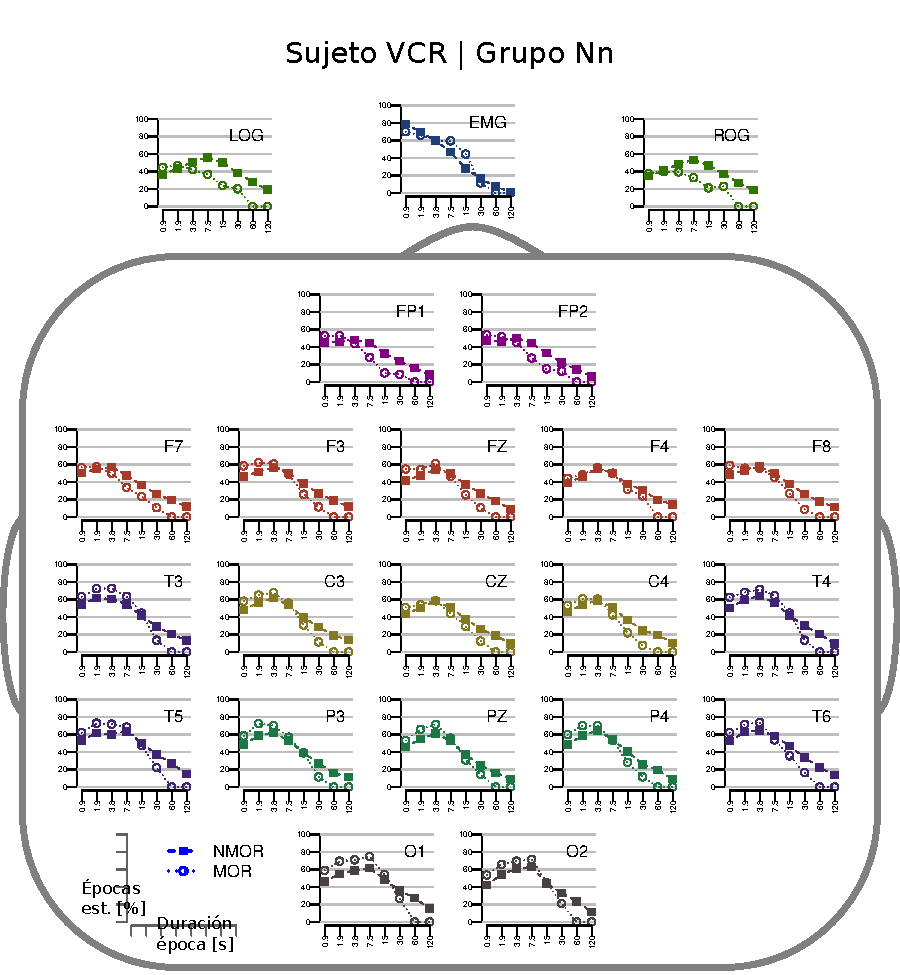
\includegraphics[width=.9\linewidth]{./img_resultados/cabeza_VCR.pdf}
%%\caption{Porcentajes de épocas estacionarias, VCR (VCNNS1)}
%\end{figure}

\begin{figure}
\centering
{\small
\begin{tabular}{lccccc}
\toprule
{\small Tamaño de} & \multicolumn{5}{c}{Grupo CTL} \\
    \cmidrule{2-6}
{\small ventana [s]}    & VCR & MJH & JAE & GHA & MFGR \\
\midrule
$30 \times 2^1$ &
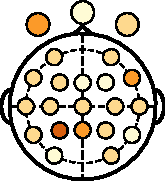
\includegraphics[width=0.13\textwidth]{./img_art_dfa/cabeza_new_VCR_60.pdf} &
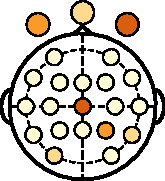
\includegraphics[width=0.13\textwidth]{./img_art_dfa/cabeza_new_MJH_60.pdf} &
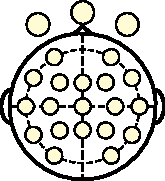
\includegraphics[width=0.13\textwidth]{./img_art_dfa/cabeza_new_JAE_60.pdf} &
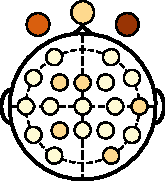
\includegraphics[width=0.13\textwidth]{./img_art_dfa/cabeza_new_GHA_60.pdf} &
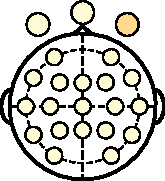
\includegraphics[width=0.13\textwidth]{./img_art_dfa/cabeza_new_MFGR_60.pdf} \\
\midrule
$30 \times 2^0$ &
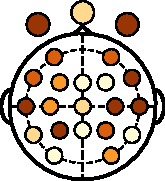
\includegraphics[width=0.13\textwidth]{./img_art_dfa/cabeza_new_VCR_30.pdf} &
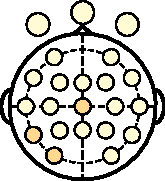
\includegraphics[width=0.13\textwidth]{./img_art_dfa/cabeza_new_MJH_30.pdf} &
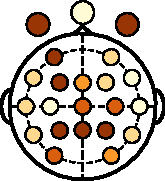
\includegraphics[width=0.13\textwidth]{./img_art_dfa/cabeza_new_JAE_30.pdf} &
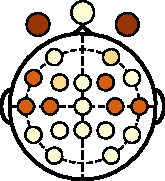
\includegraphics[width=0.13\textwidth]{./img_art_dfa/cabeza_new_GHA_30.pdf} &
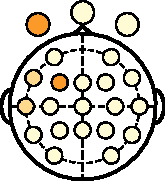
\includegraphics[width=0.13\textwidth]{./img_art_dfa/cabeza_new_MFGR_30.pdf} \\
\midrule
$30 \times 2^{-1}$ &
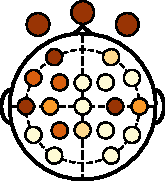
\includegraphics[width=0.13\textwidth]{./img_art_dfa/cabeza_new_VCR_15.pdf} &
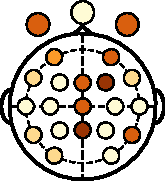
\includegraphics[width=0.13\textwidth]{./img_art_dfa/cabeza_new_MJH_15.pdf} &
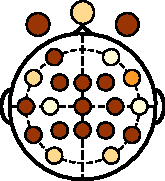
\includegraphics[width=0.13\textwidth]{./img_art_dfa/cabeza_new_JAE_15.pdf} &
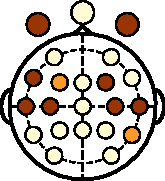
\includegraphics[width=0.13\textwidth]{./img_art_dfa/cabeza_new_GHA_15.pdf} &
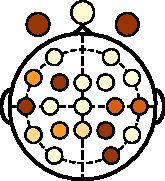
\includegraphics[width=0.13\textwidth]{./img_art_dfa/cabeza_new_MFGR_15.pdf} \\
\bottomrule
\end{tabular}\\

\includegraphics[scale=.7]{./img_art_dfa/escala.pdf} \\
}
\end{figure}

\begin{figure}
\centering
{\small
\begin{tabular}{lccccc}
\toprule
{ Tamaño de} & \multicolumn{5}{c}{Grupo PDC} \\
    \cmidrule{2-6}
{ ventana [s]}    & CLO & RLO & RRU & JGZ & AEFP \\
\midrule
$30 \times 2^1$ &
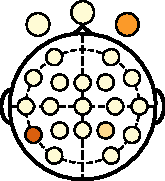
\includegraphics[width=0.13\textwidth]{./img_art_dfa/cabeza_new_CLO_60.pdf} &
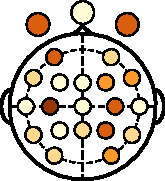
\includegraphics[width=0.13\textwidth]{./img_art_dfa/cabeza_new_RLO_60.pdf} &
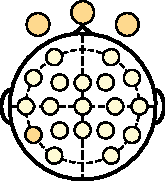
\includegraphics[width=0.13\textwidth]{./img_art_dfa/cabeza_new_RRU_60.pdf} &
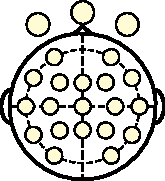
\includegraphics[width=0.13\textwidth]{./img_art_dfa/cabeza_new_JGZ_60.pdf} &
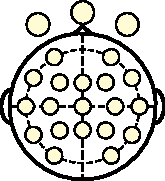
\includegraphics[width=0.13\textwidth]{./img_art_dfa/cabeza_new_AEFP_60.pdf} \\
\midrule
$30 \times 2^0$ &
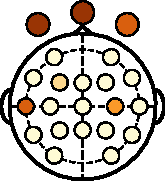
\includegraphics[width=0.13\textwidth]{./img_art_dfa/cabeza_new_CLO_30.pdf} &
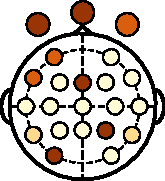
\includegraphics[width=0.13\textwidth]{./img_art_dfa/cabeza_new_RLO_30.pdf} &
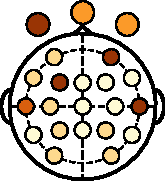
\includegraphics[width=0.13\textwidth]{./img_art_dfa/cabeza_new_RRU_30.pdf} &
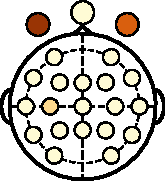
\includegraphics[width=0.13\textwidth]{./img_art_dfa/cabeza_new_JGZ_30.pdf} &
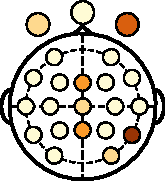
\includegraphics[width=0.13\textwidth]{./img_art_dfa/cabeza_new_AEFP_30.pdf} \\
\midrule
$30 \times 2^{-1}$ &
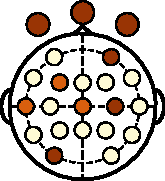
\includegraphics[width=0.13\textwidth]{./img_art_dfa/cabeza_new_CLO_15.pdf} &
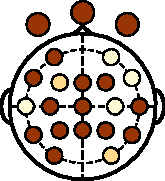
\includegraphics[width=0.13\textwidth]{./img_art_dfa/cabeza_new_RLO_15.pdf} &
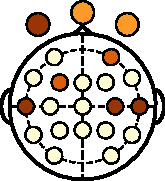
\includegraphics[width=0.13\textwidth]{./img_art_dfa/cabeza_new_RRU_15.pdf} &
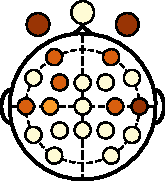
\includegraphics[width=0.13\textwidth]{./img_art_dfa/cabeza_new_JGZ_15.pdf} &
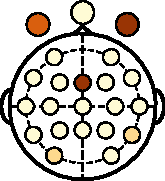
\includegraphics[width=0.13\textwidth]{./img_art_dfa/cabeza_new_AEFP_15.pdf} \\
\bottomrule
\end{tabular} \\

\includegraphics[scale=.7]{./img_art_dfa/escala.pdf} \\
}
\caption{Regiones donde la cantidad  de ventanas estacionarias es significativamente diferente
durante MOR y NMOR. Diferentes tamaños de ventana}
\end{figure}

%%%%%%%%%%%%%%%%%%%%%%%%%%%%%%%%%%%%%%%%%%%%%%%%%%%%%%%%%%%%%%%%%%%%%%%%%%%%%%%%%%%%%%%%%%%%%%%%%%%
%%%%%%%%%%%%%%%%%%%%%%%%%%%%%%%%%%%%%%%%%%%%%%%%%%%%%%%%%%%%%%%%%%%%%%%%%%%%%%%%%%%%%%%%%%%%%%%%%%%

\begin{figure}
\begin{subfigure}{\textwidth}
\centering
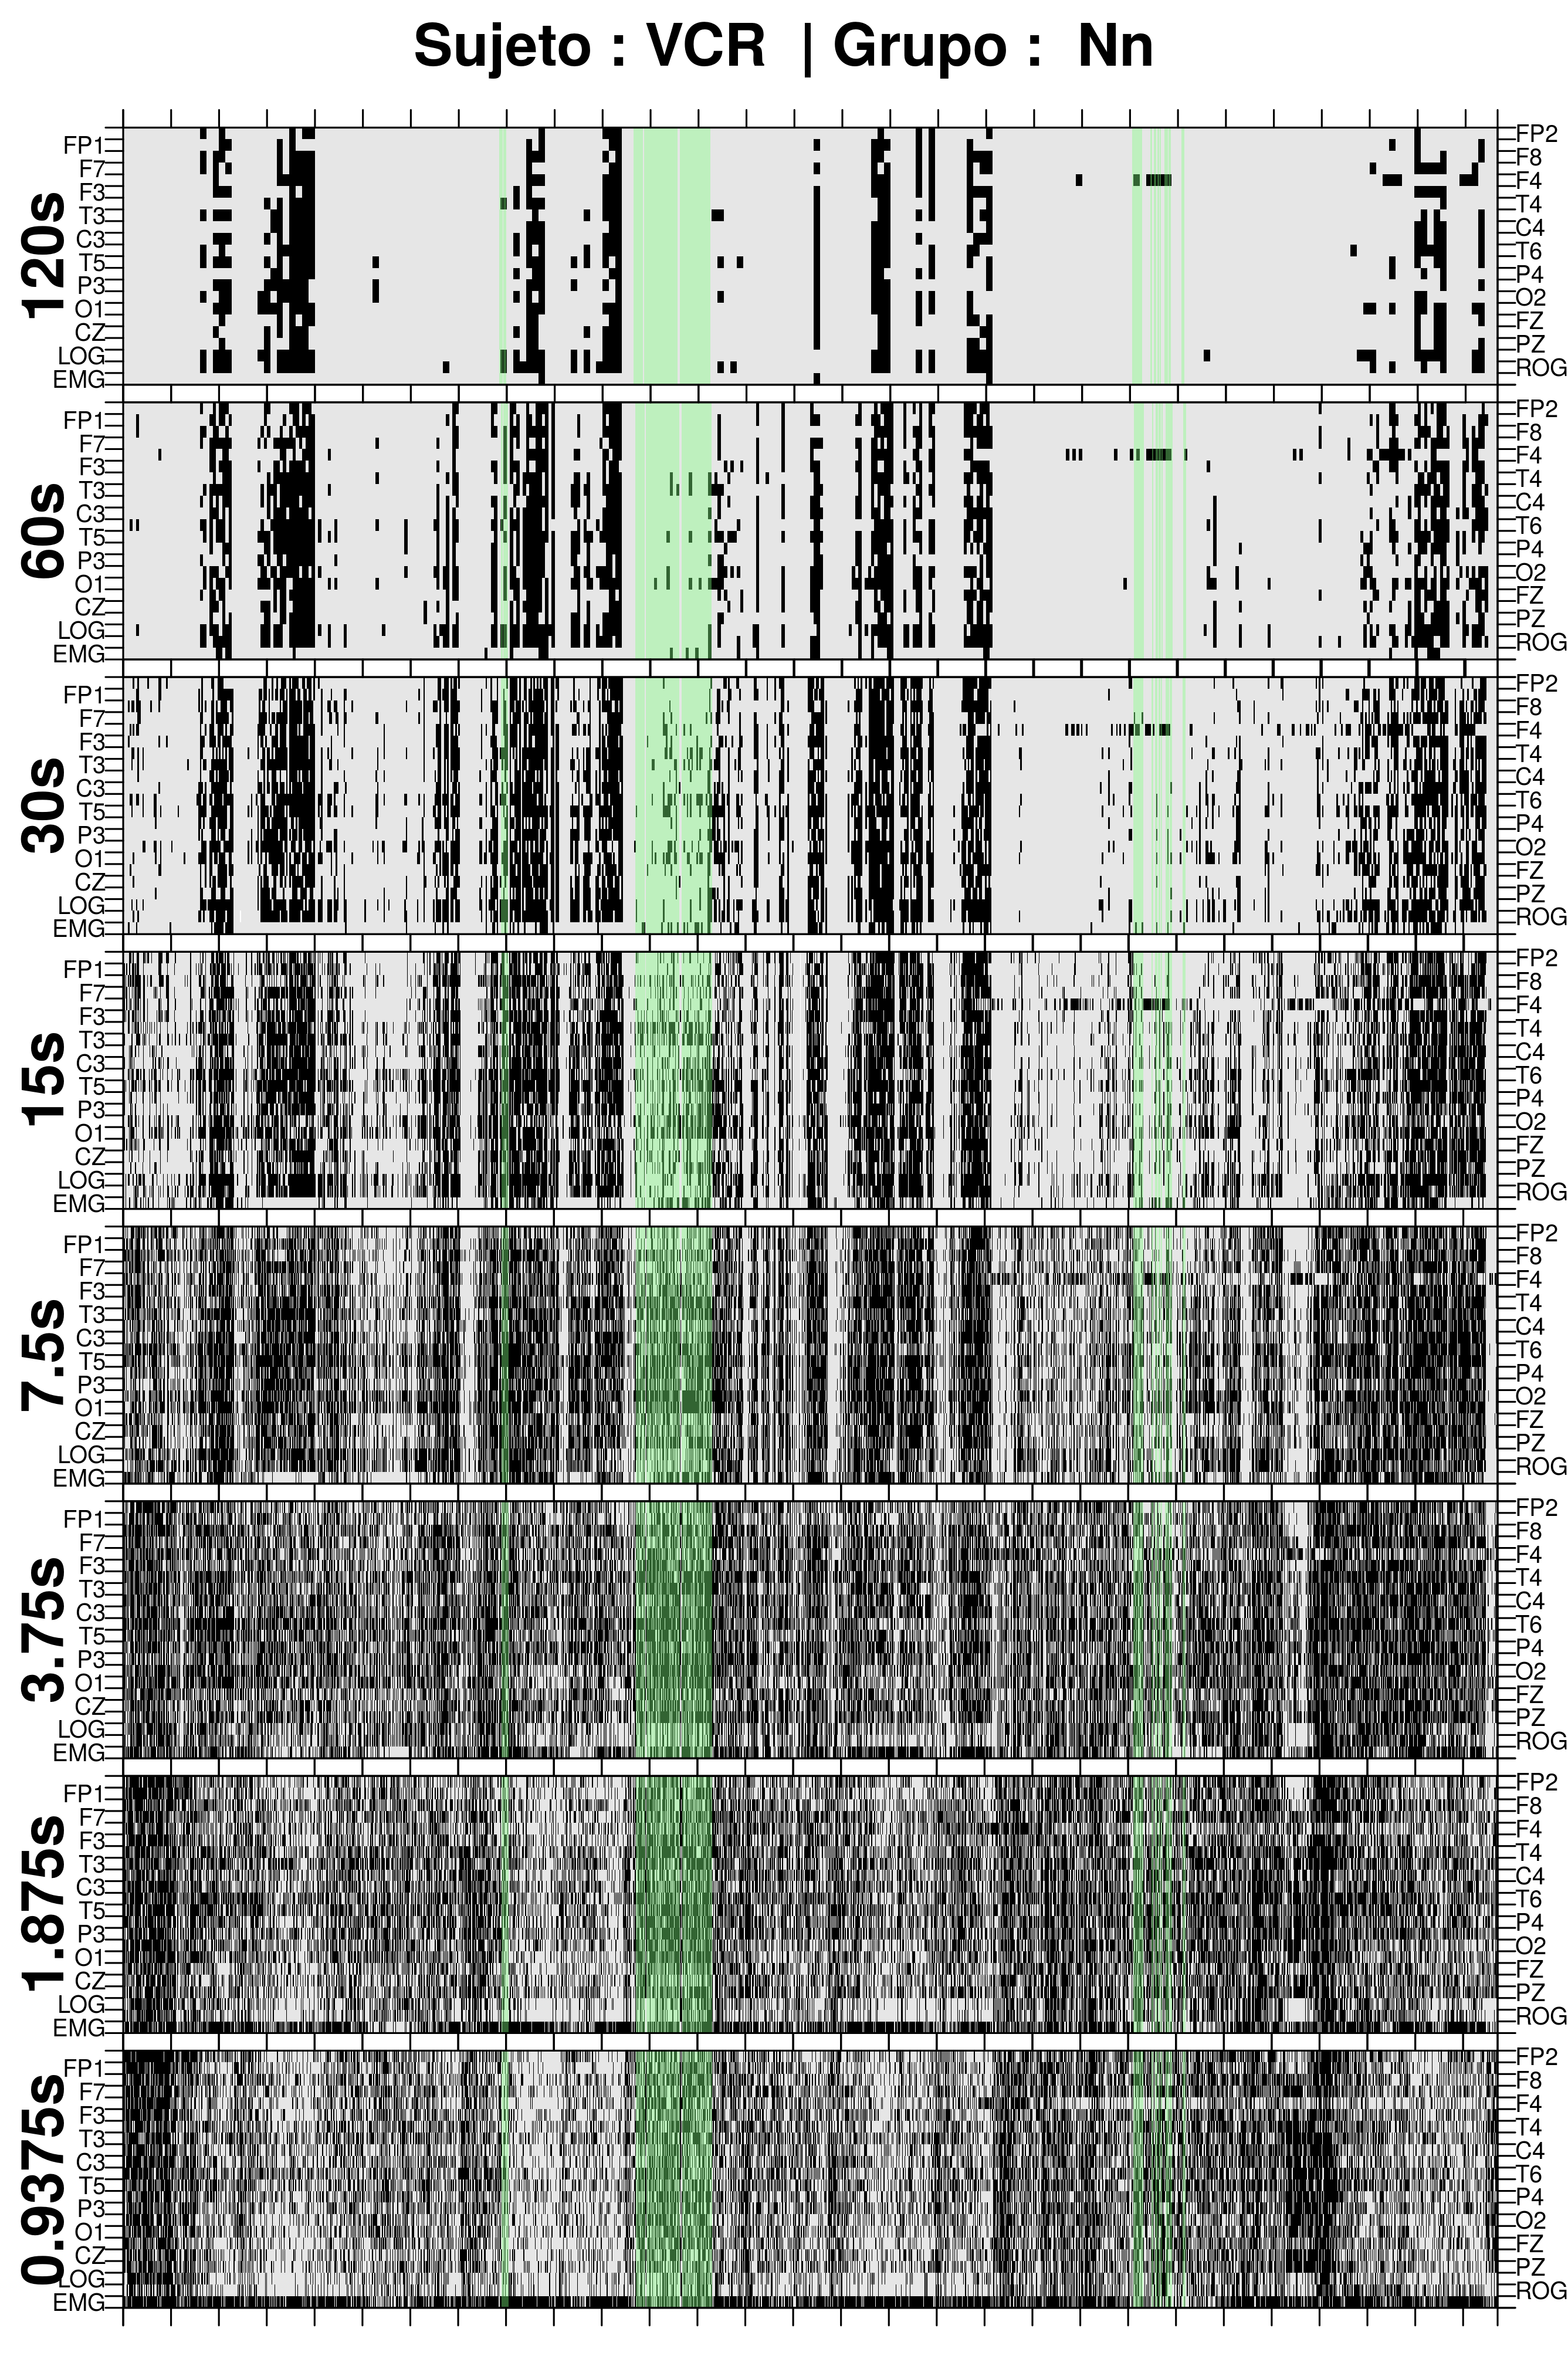
\includegraphics[width=0.9\linewidth]
{./img_ejemplos/VCNNS1_comp_est_.png} 
\caption{Épocas estacionarias usando diferentes tamaños de ventana}
\end{subfigure}
\end{figure}

\begin{figure}
\ContinuedFloat
\begin{subfigure}{\linewidth}
\centering
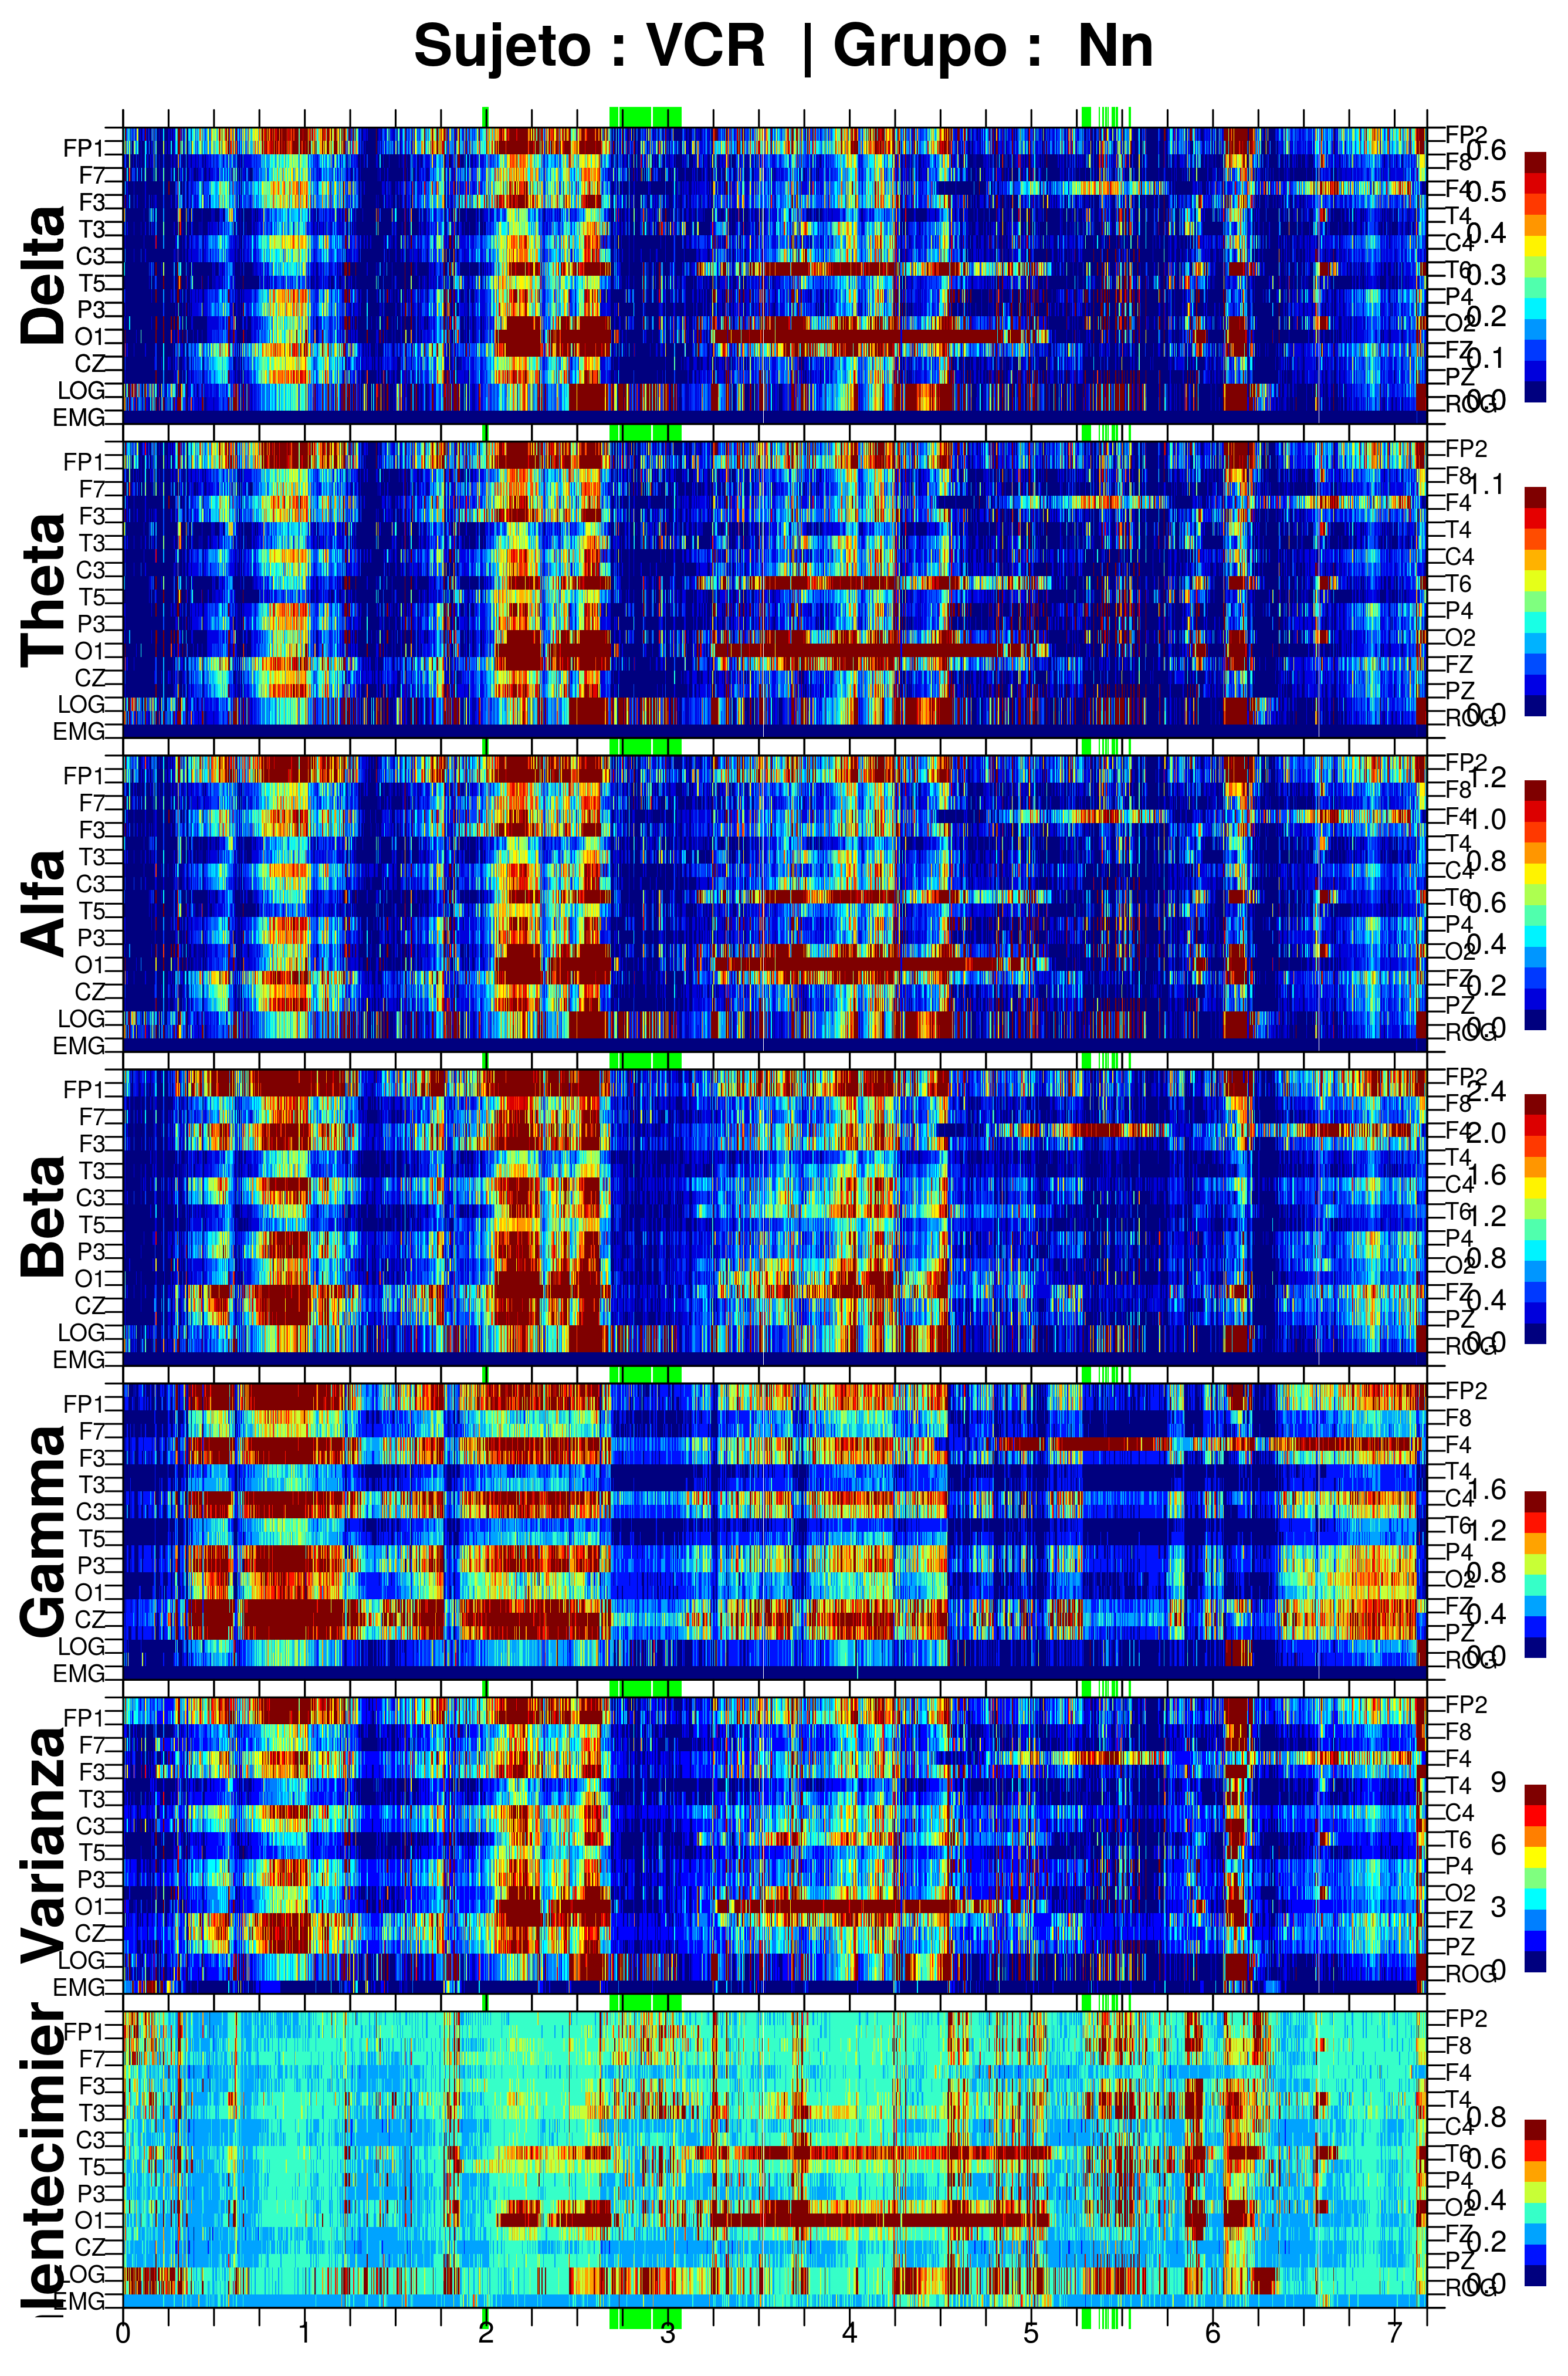
\includegraphics[width=0.9\linewidth]
{./enlentecimiento/VCNNS1_espectral_total.png} 
\caption{Espectro de potencias de banda ancha}
\end{subfigure}
\end{figure}

\begin{figure}
\ContinuedFloat
\begin{subfigure}{\linewidth}
\centering
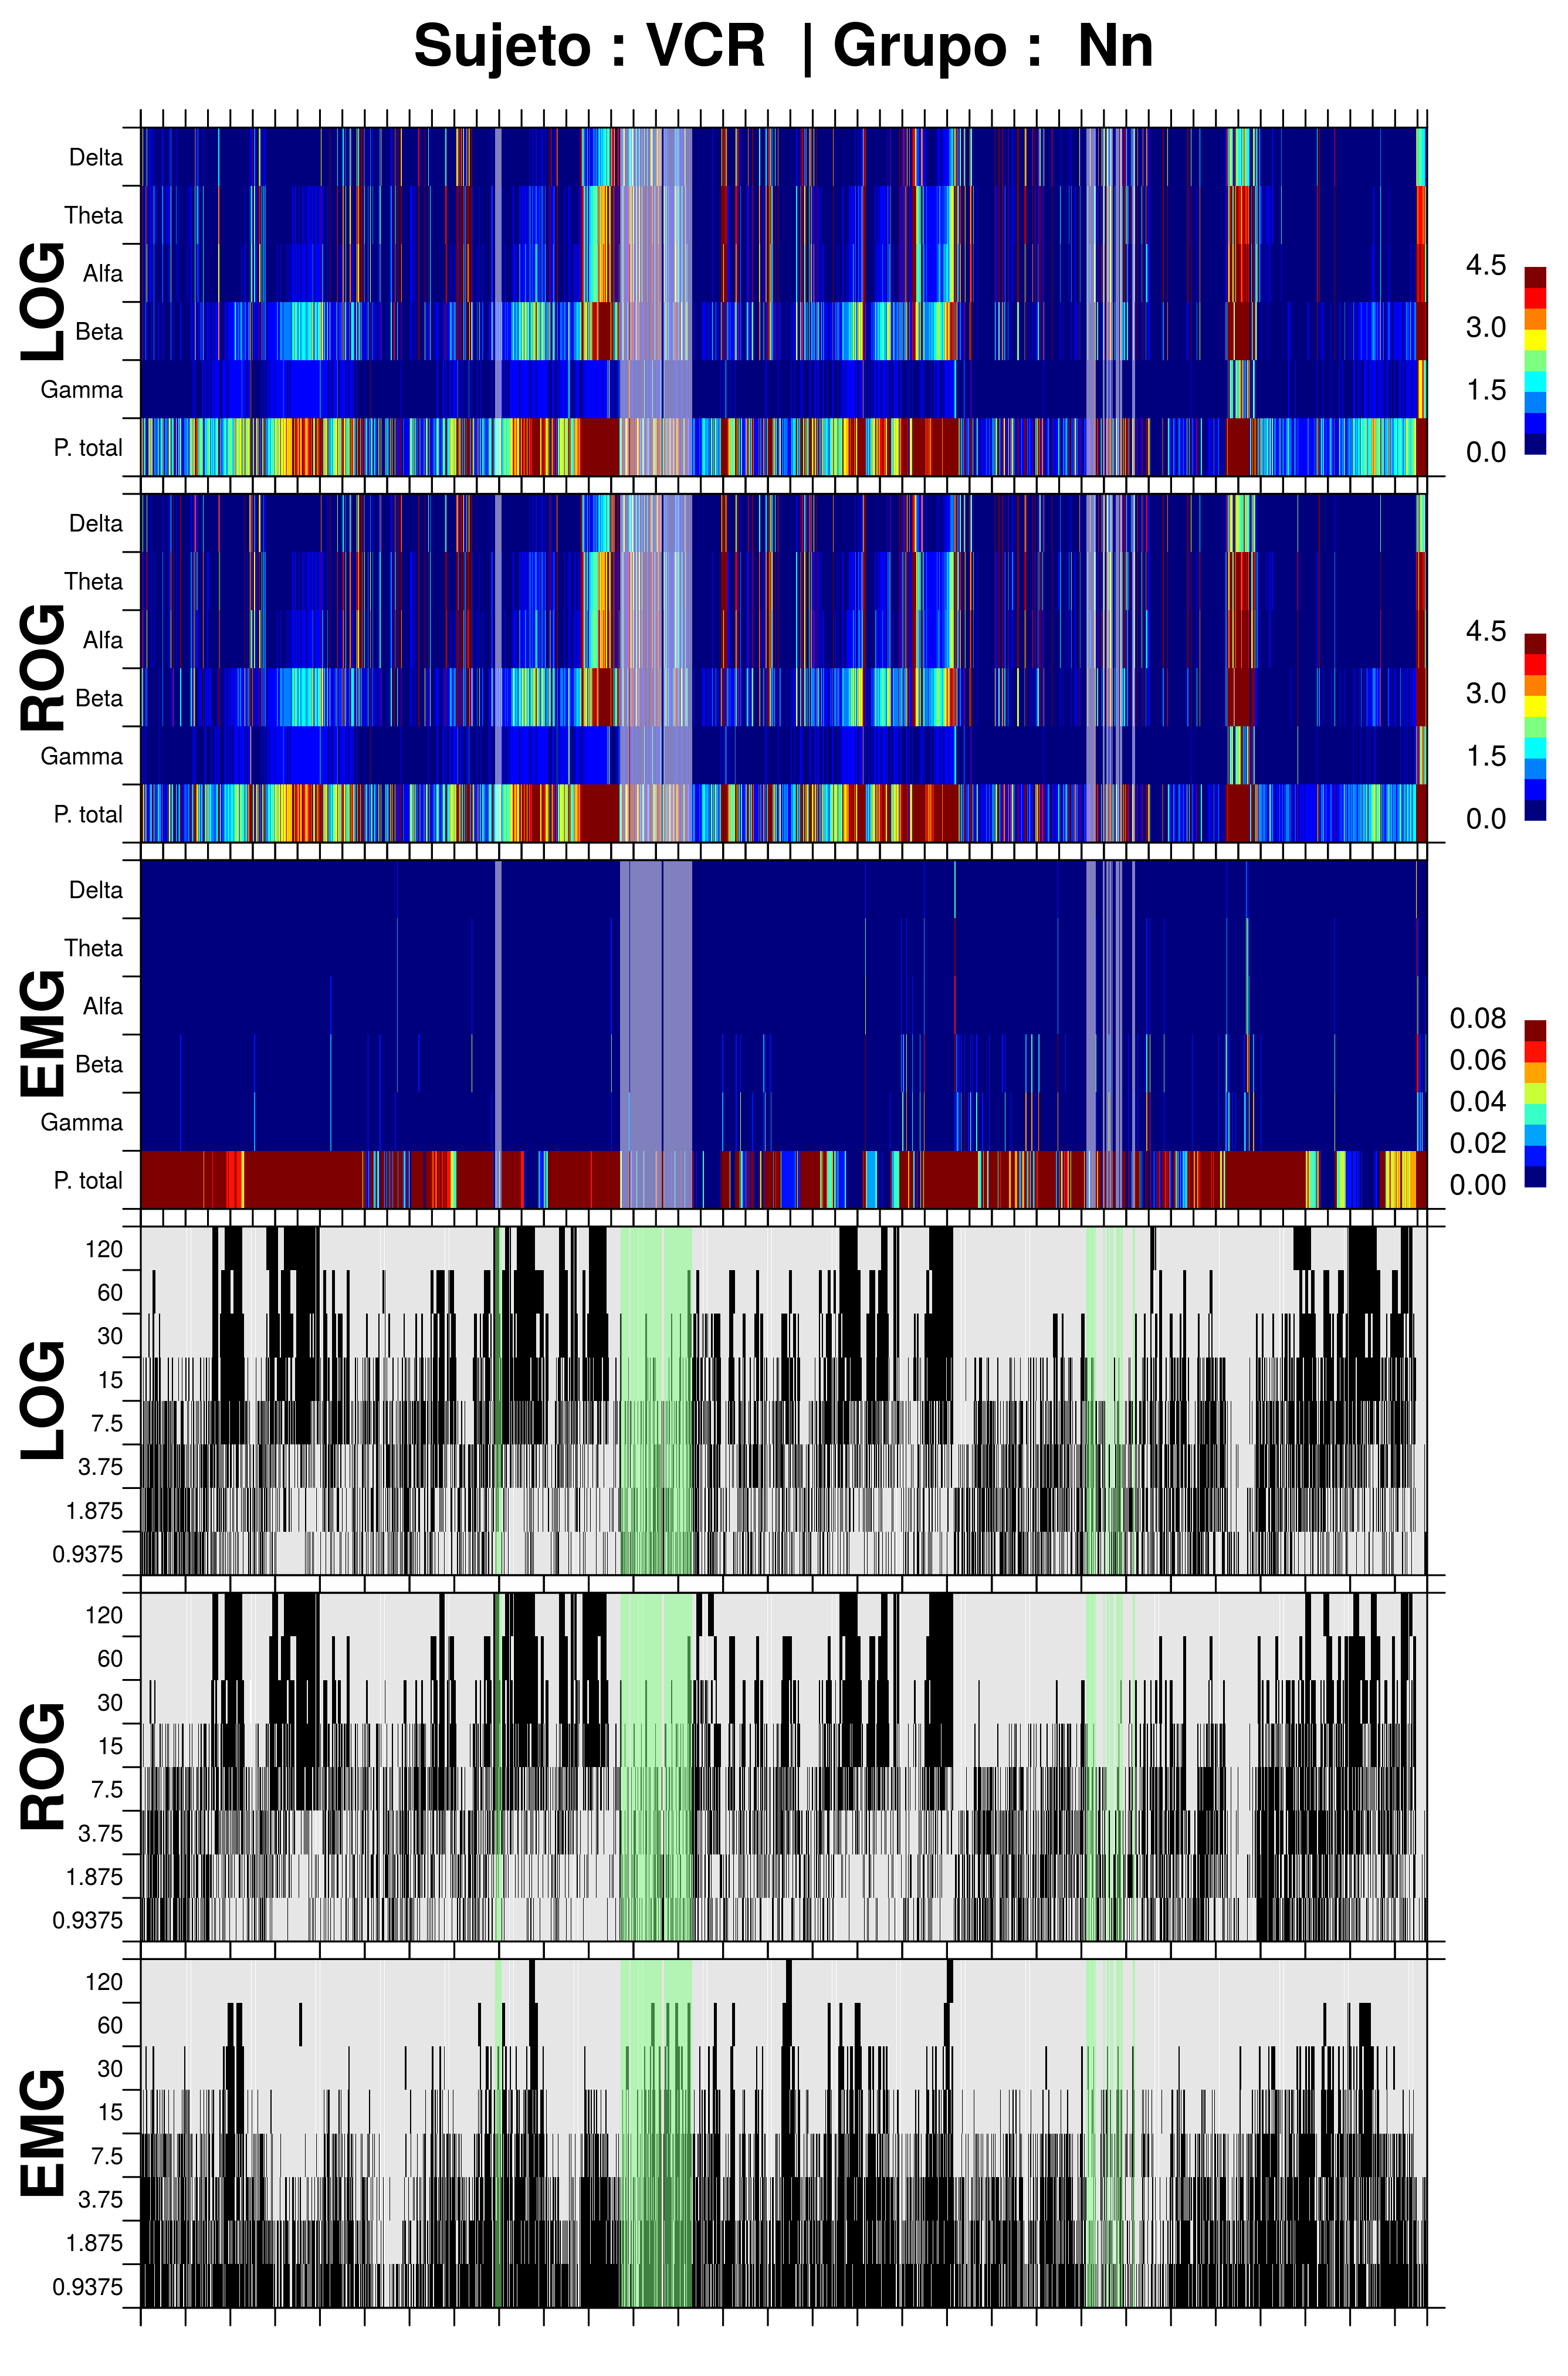
\includegraphics[width=0.9\linewidth]
{./img_resultados/VCNNS1_combinado_.png} 
\caption{Espectro de potencias y análisis de estacionariedad para los canales LOG, ROG y EMG}
\end{subfigure}
\end{figure}

\begin{figure}
\ContinuedFloat
\begin{subfigure}{\linewidth}
\centering
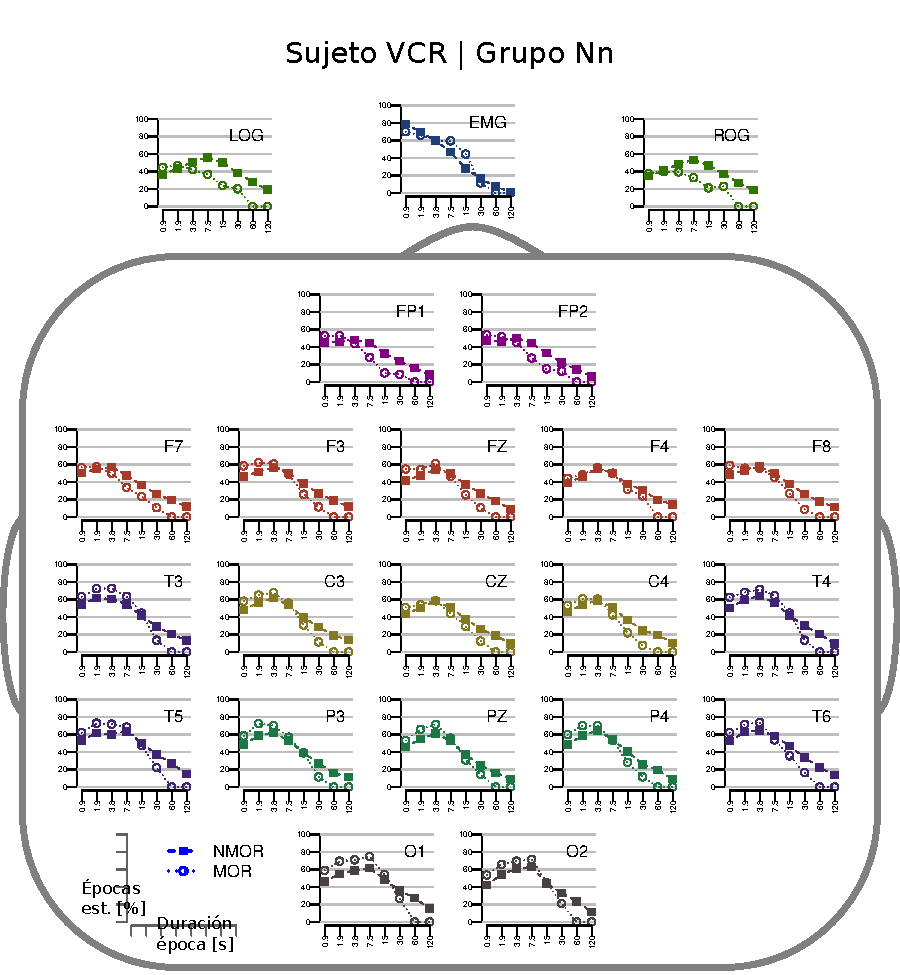
\includegraphics[width=.9\linewidth]{./img_resultados/cabeza_VCR.pdf}
%\caption{Porcentajes de épocas estacionarias, VCR (VCNNS1)}
\caption{Resumen de épocas estacionarias según tamaño de ventana}
\end{subfigure}
\caption{Gráficos individuales para el sujeto VCR}
\end{figure}

%%%%%%%%%%%%%%%%%%%%%%%%%%%%%%%%%%%%%%%%%%%%%%%%%

\begin{figure}
\centering
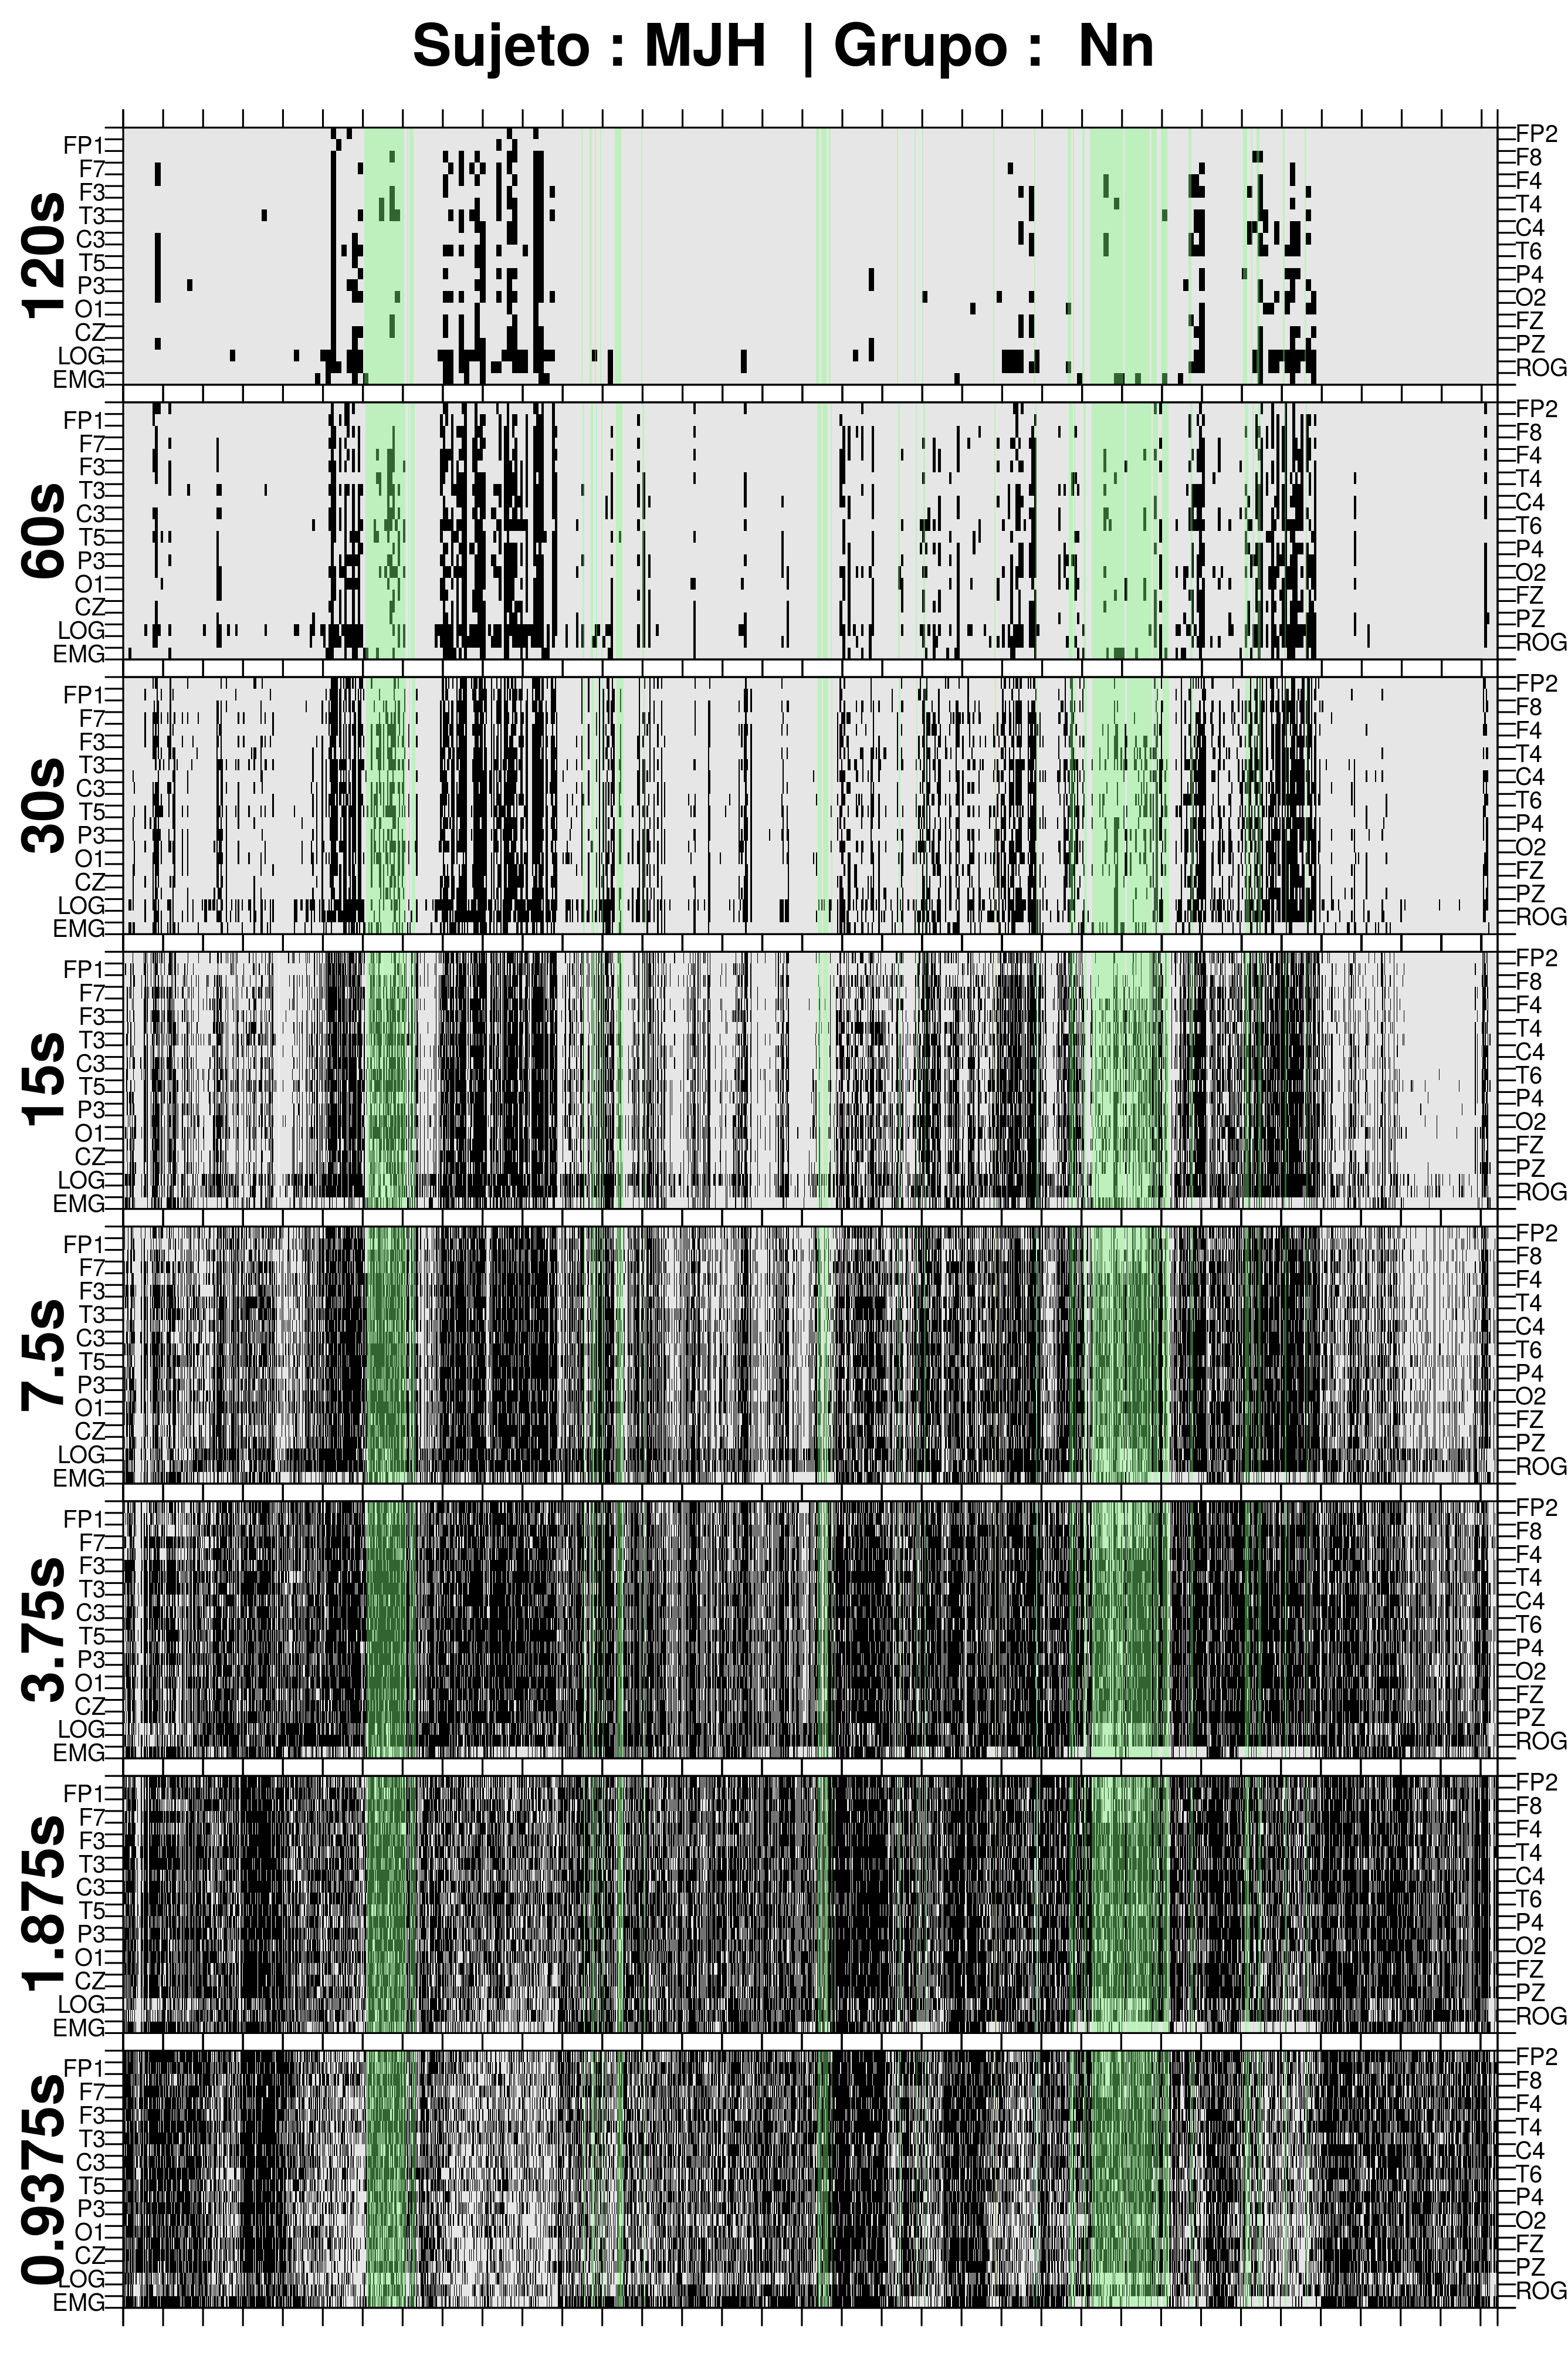
\includegraphics[width=0.9\linewidth]
{./img_ejemplos/MJNNVIGILOS_comp_est_.png} 
\end{figure}

\begin{figure}
\centering
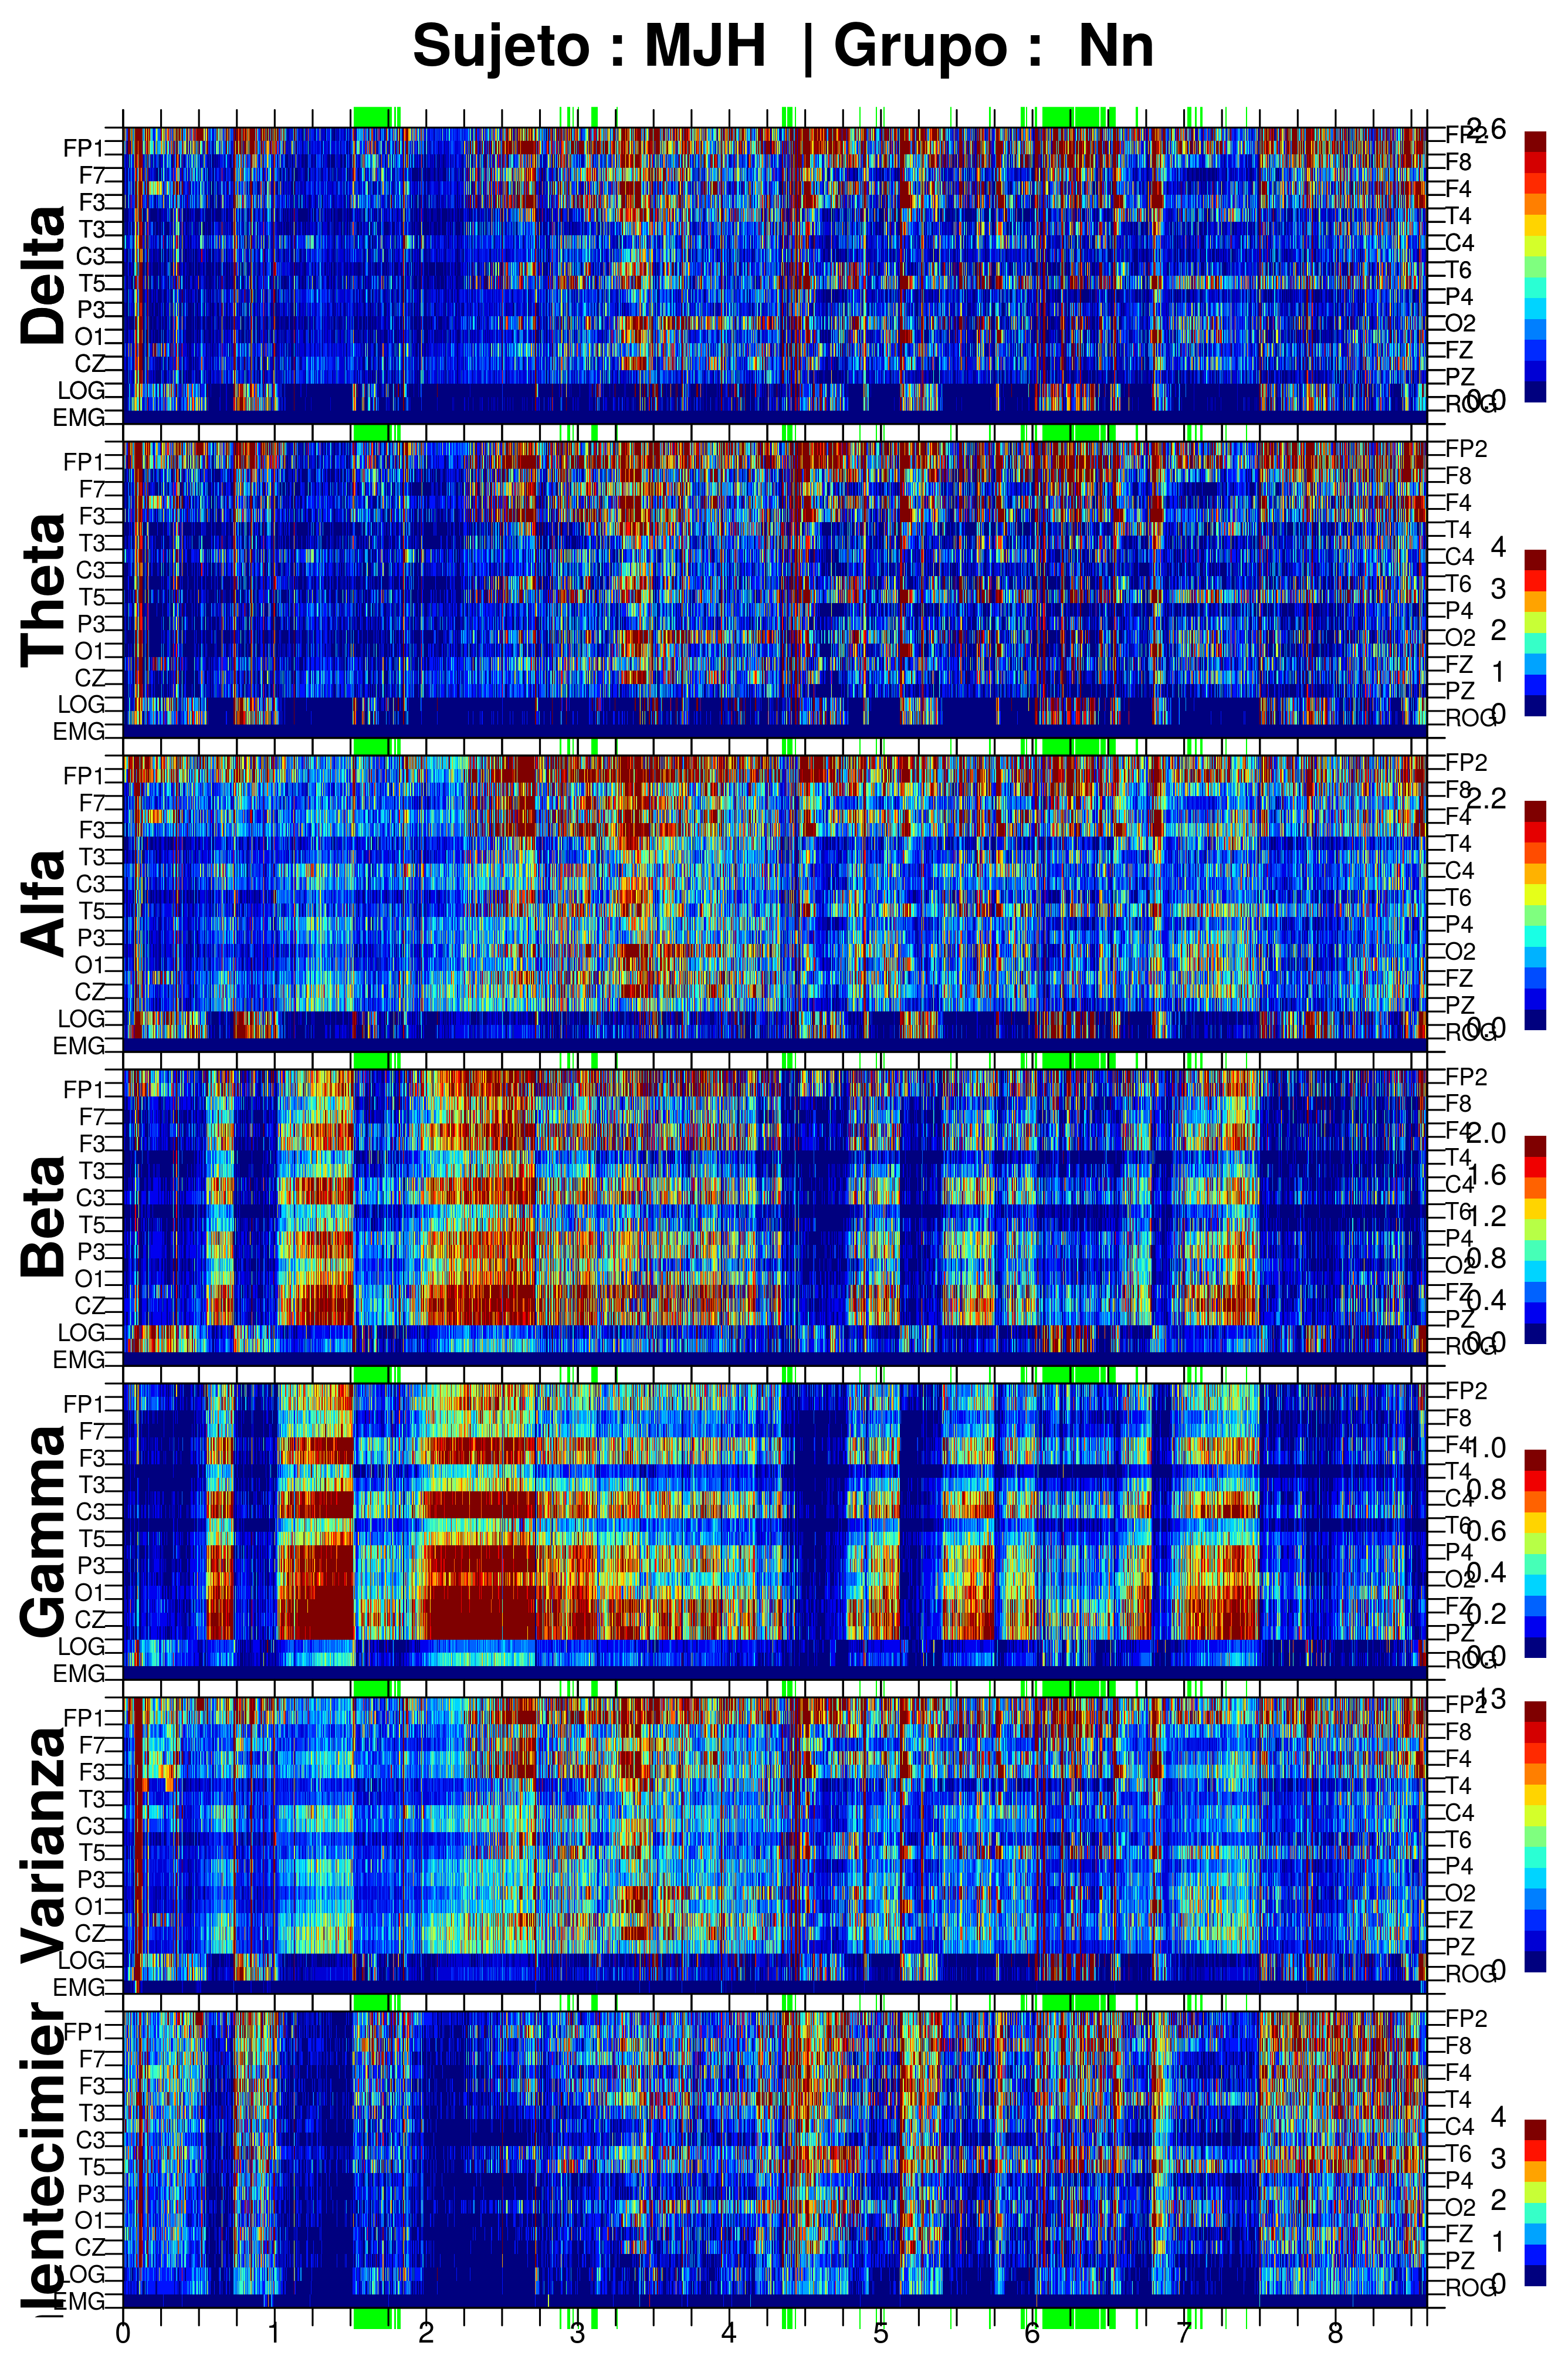
\includegraphics[width=0.9\linewidth]
{./enlentecimiento/MJNNVIGILOS_espectral_total.png} 
\end{figure}

\begin{figure}
\centering
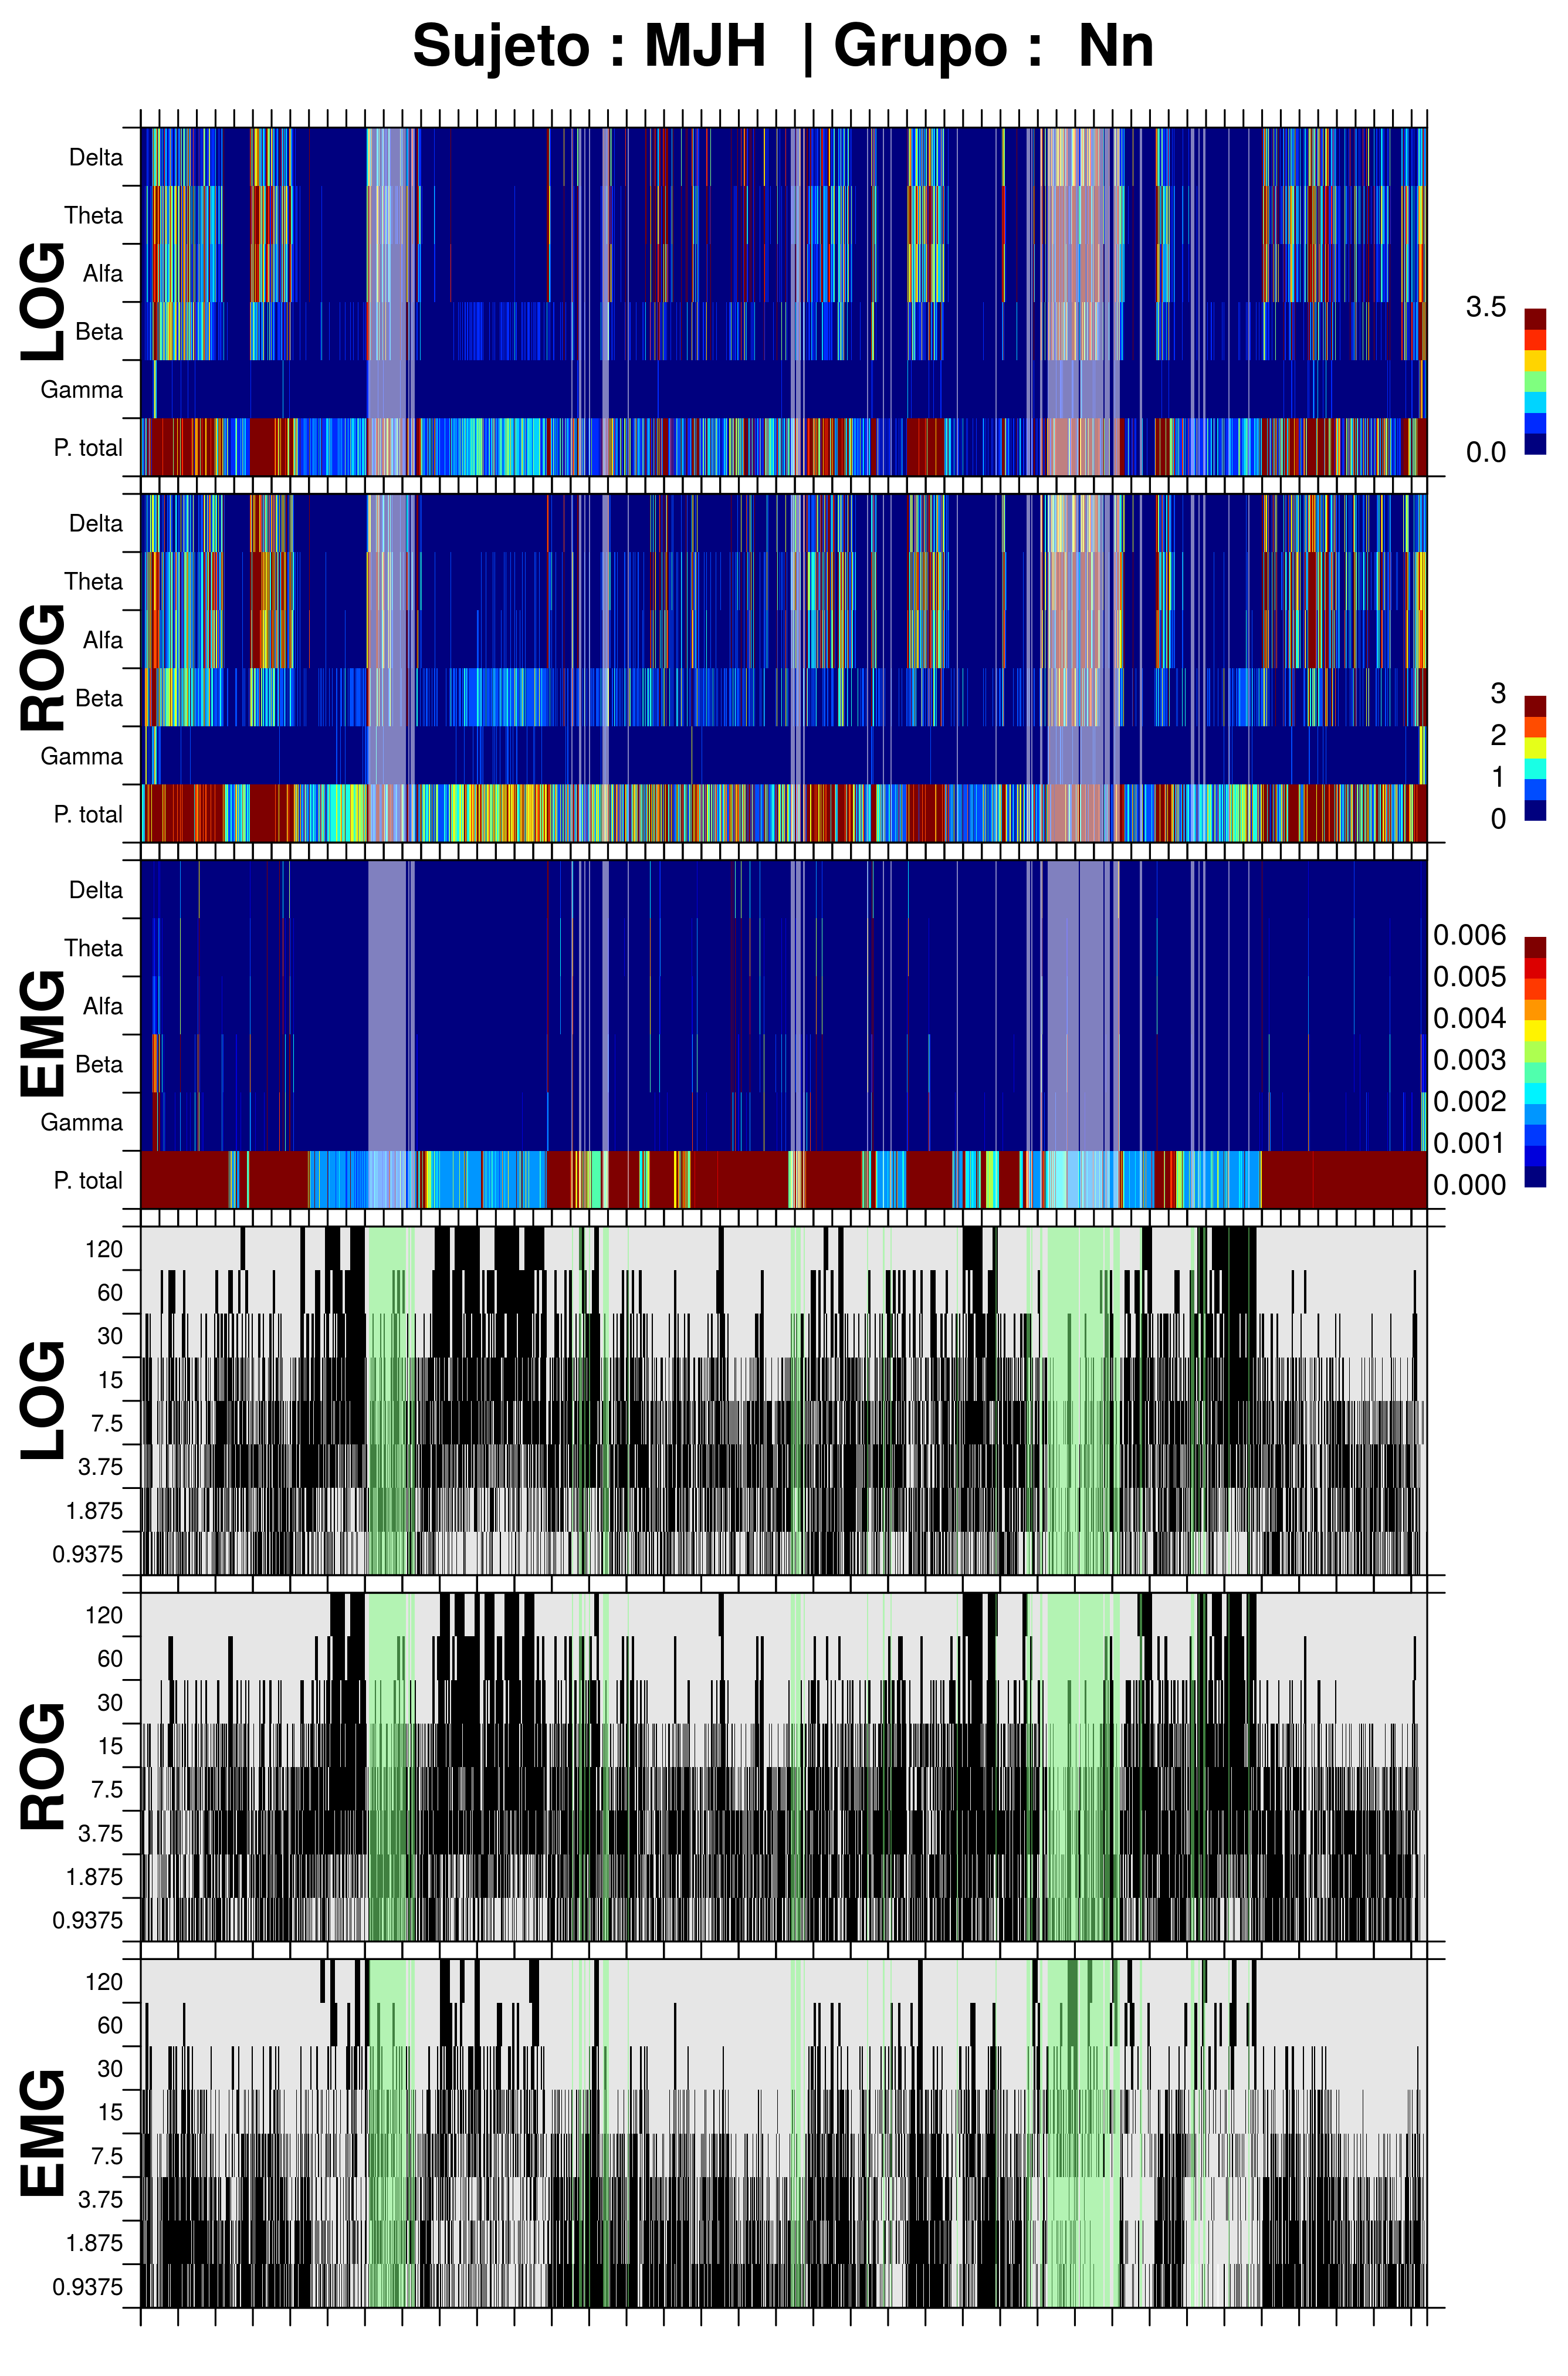
\includegraphics[width=0.9\linewidth]
{./img_resultados/MJNNVIGILOS_combinado_.png} 
\end{figure}

\begin{figure}
\centering
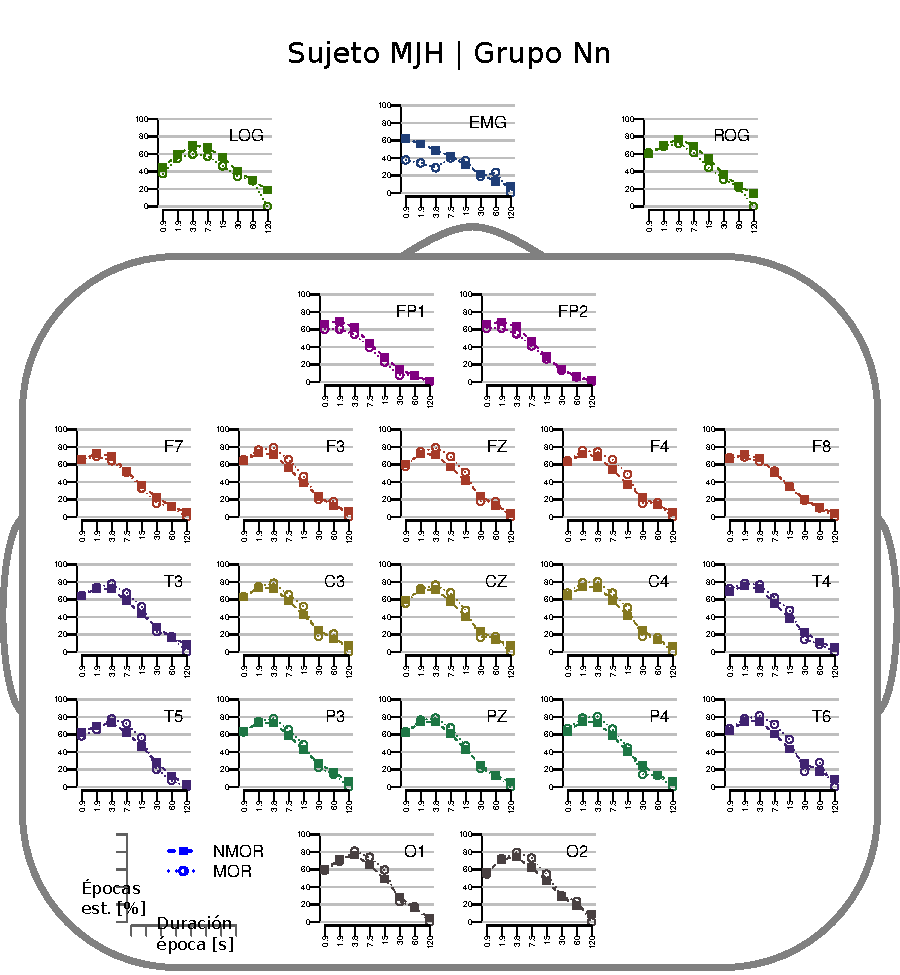
\includegraphics[width=.9\linewidth]{./img_resultados/cabeza_MJH.pdf}
%\caption{Porcentajes de épocas estacionarias, MJH (MJNNVIGILOS)}
\end{figure}

%%%%%%%%%%%%%%%%%%%%%%%%%%%%%%%%%%%%%%%%%%%%%%%%%

\begin{figure}
\centering
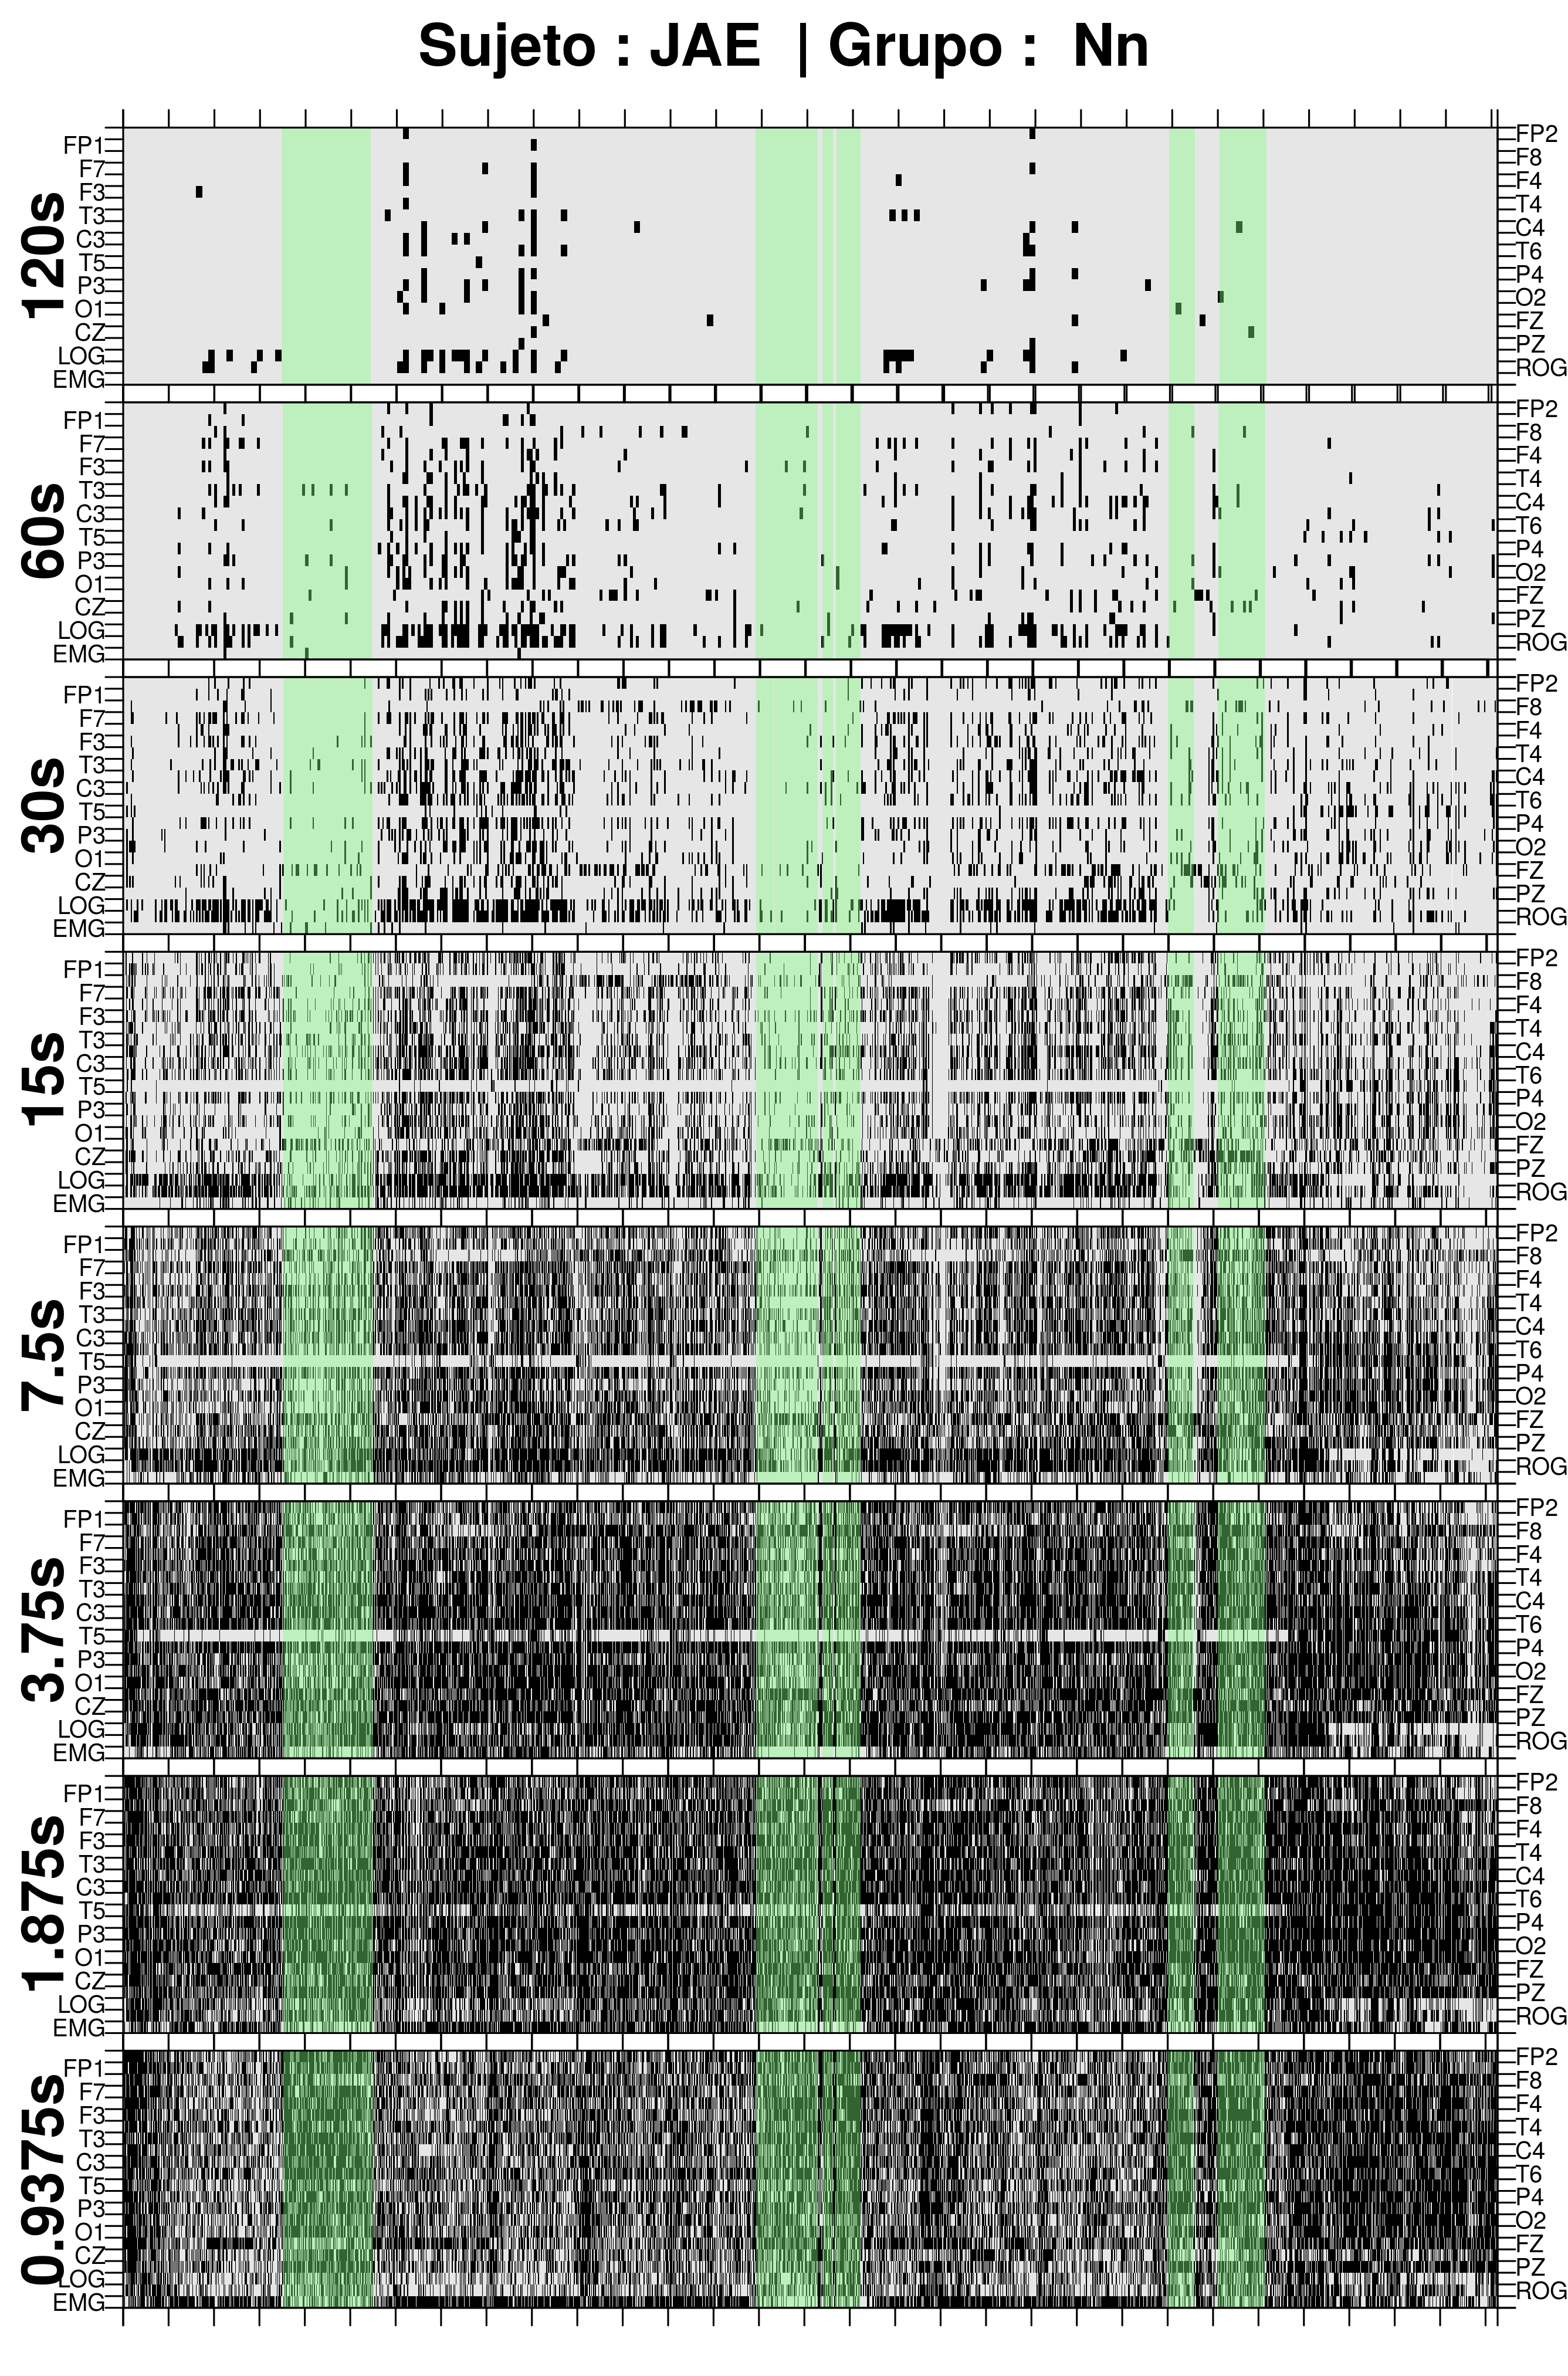
\includegraphics[width=0.9\linewidth]
{./img_ejemplos/JANASUE_comp_est_.png} 
\end{figure}
\begin{figure}
\centering
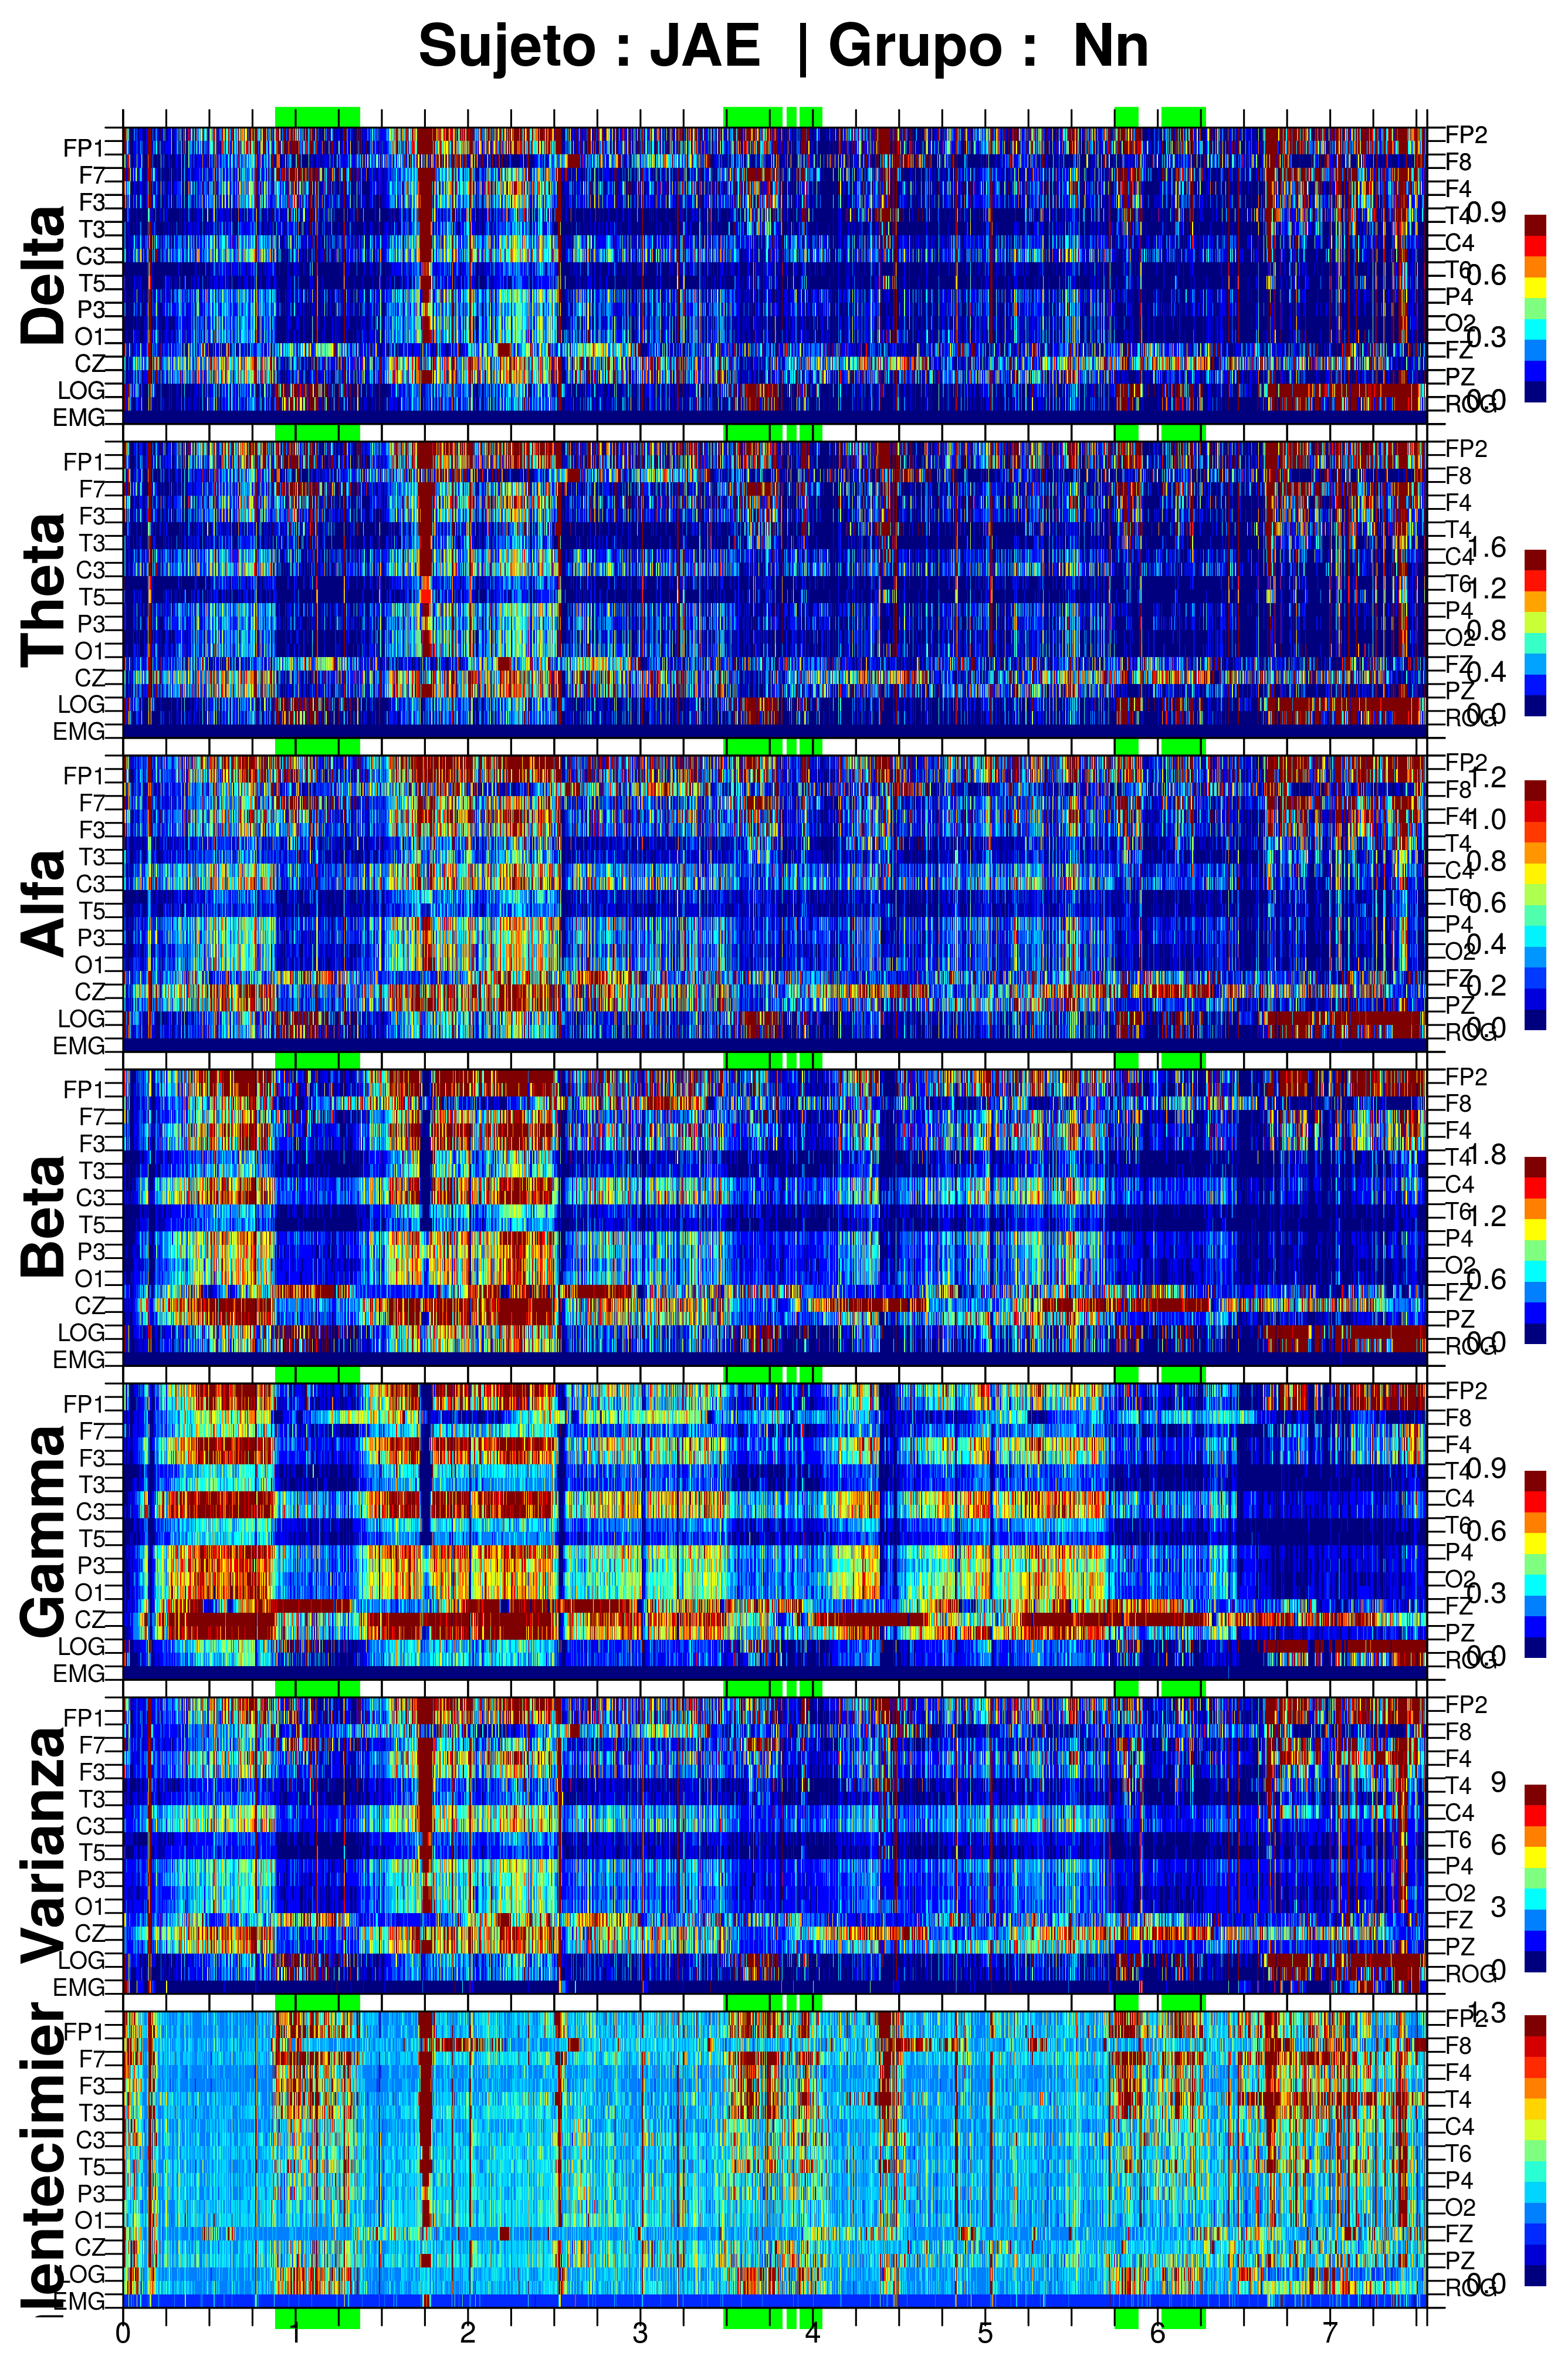
\includegraphics[width=0.9\linewidth]
{./enlentecimiento/JANASUE_espectral_total.png} 
\end{figure}
\begin{figure}
\centering
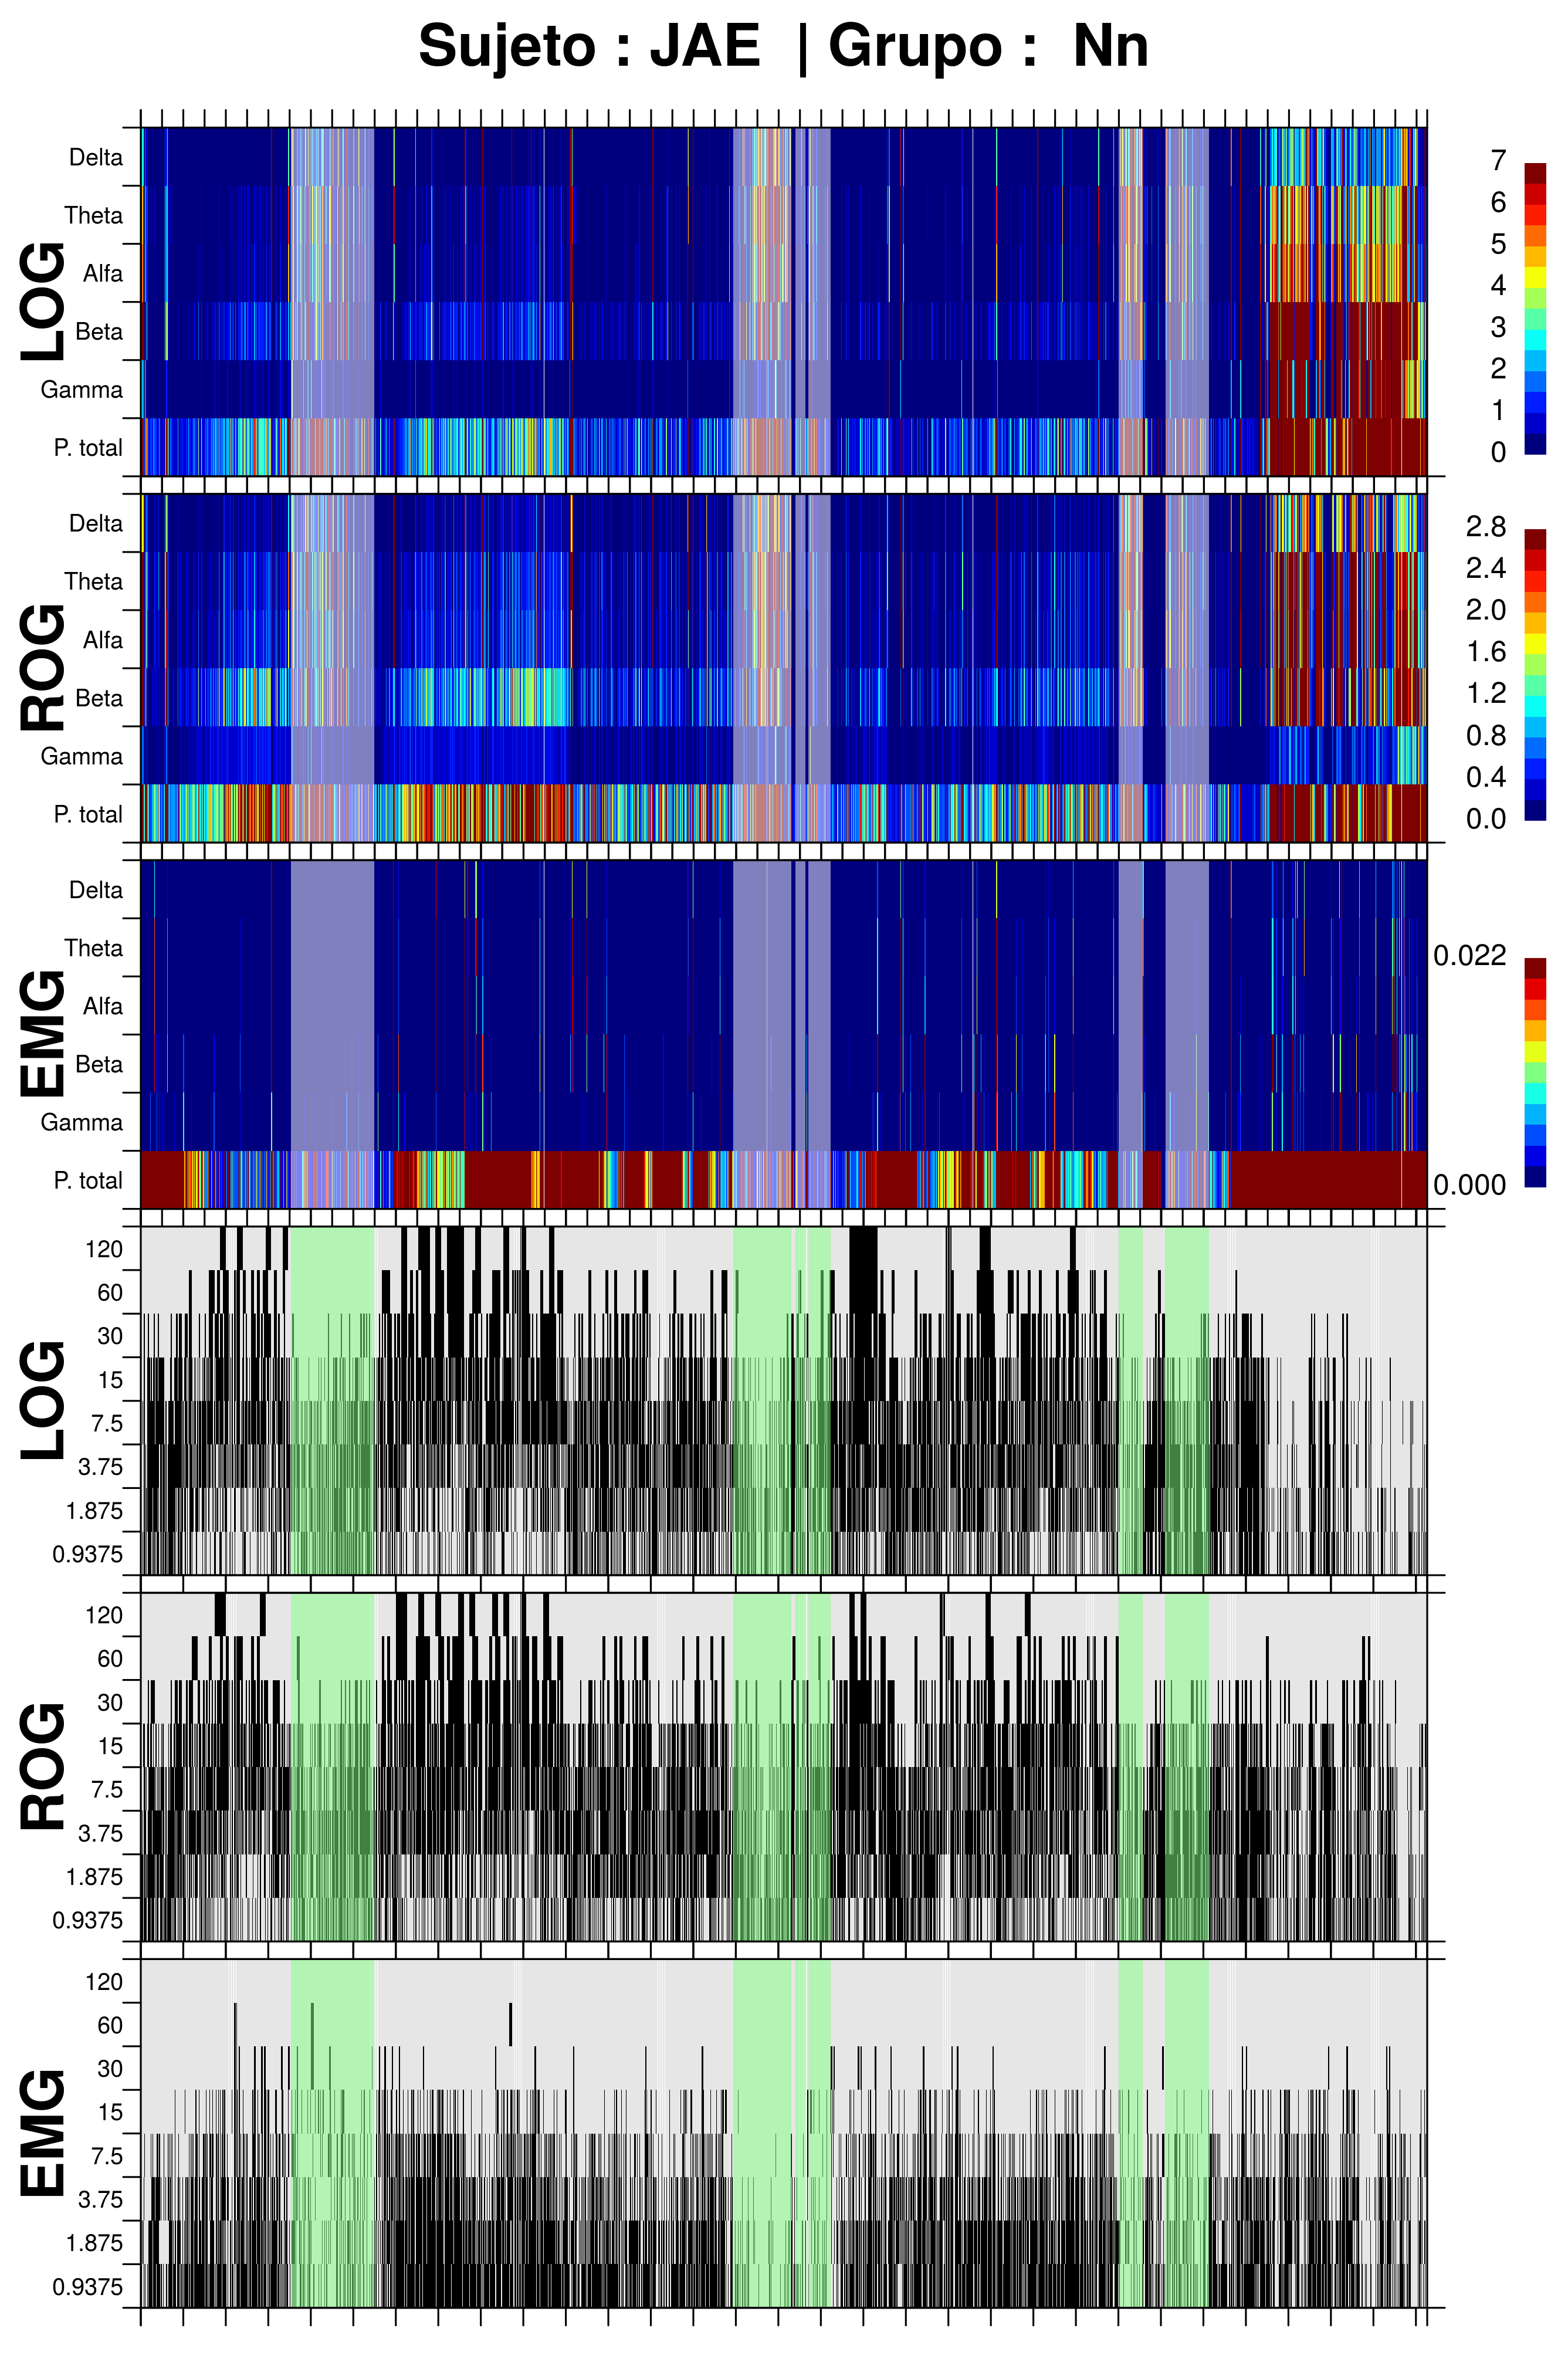
\includegraphics[width=0.9\linewidth]
{./img_resultados/JANASUE_combinado_.png} 
\end{figure}

\begin{figure}
\centering
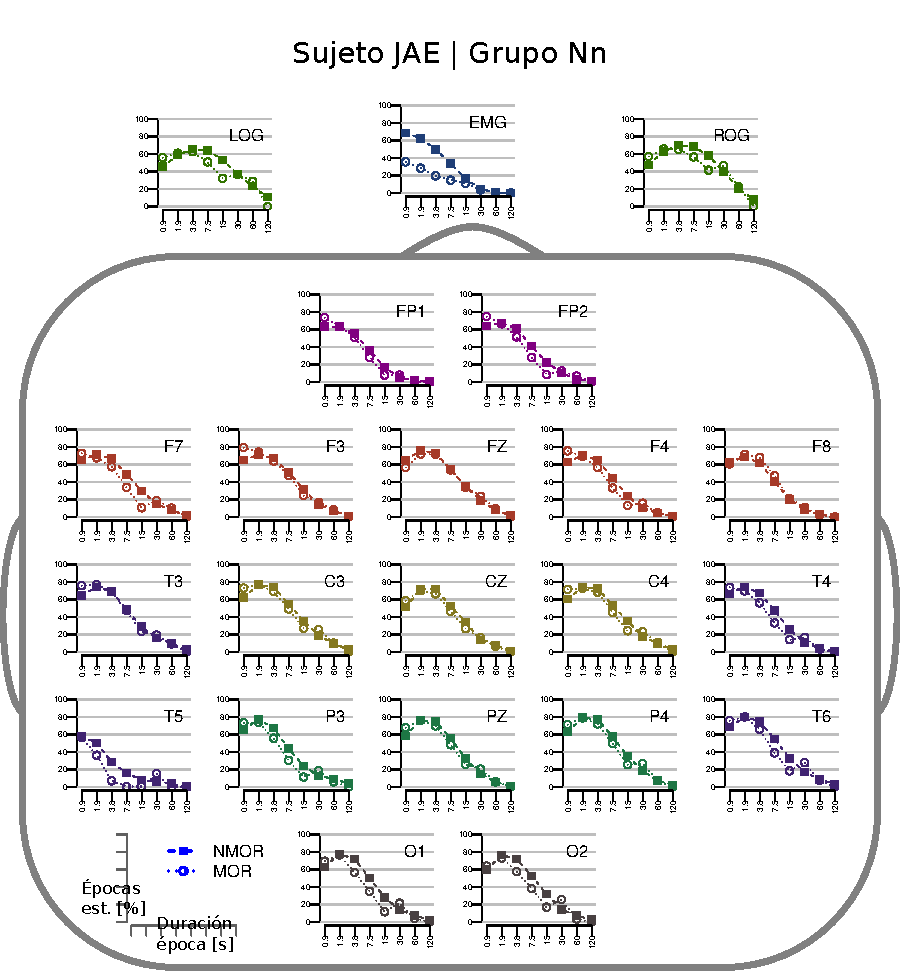
\includegraphics[width=.9\linewidth]{./img_resultados/cabeza_JAE.pdf}
%\caption{Porcentajes de épocas estacionarias, JAE (JANASUE)}
\end{figure}

%%%%%%%%%%%%%%%%%%%%%%%%%%%%%%%%%%%%%%%%%%%%%%%%%

\begin{figure}
\centering
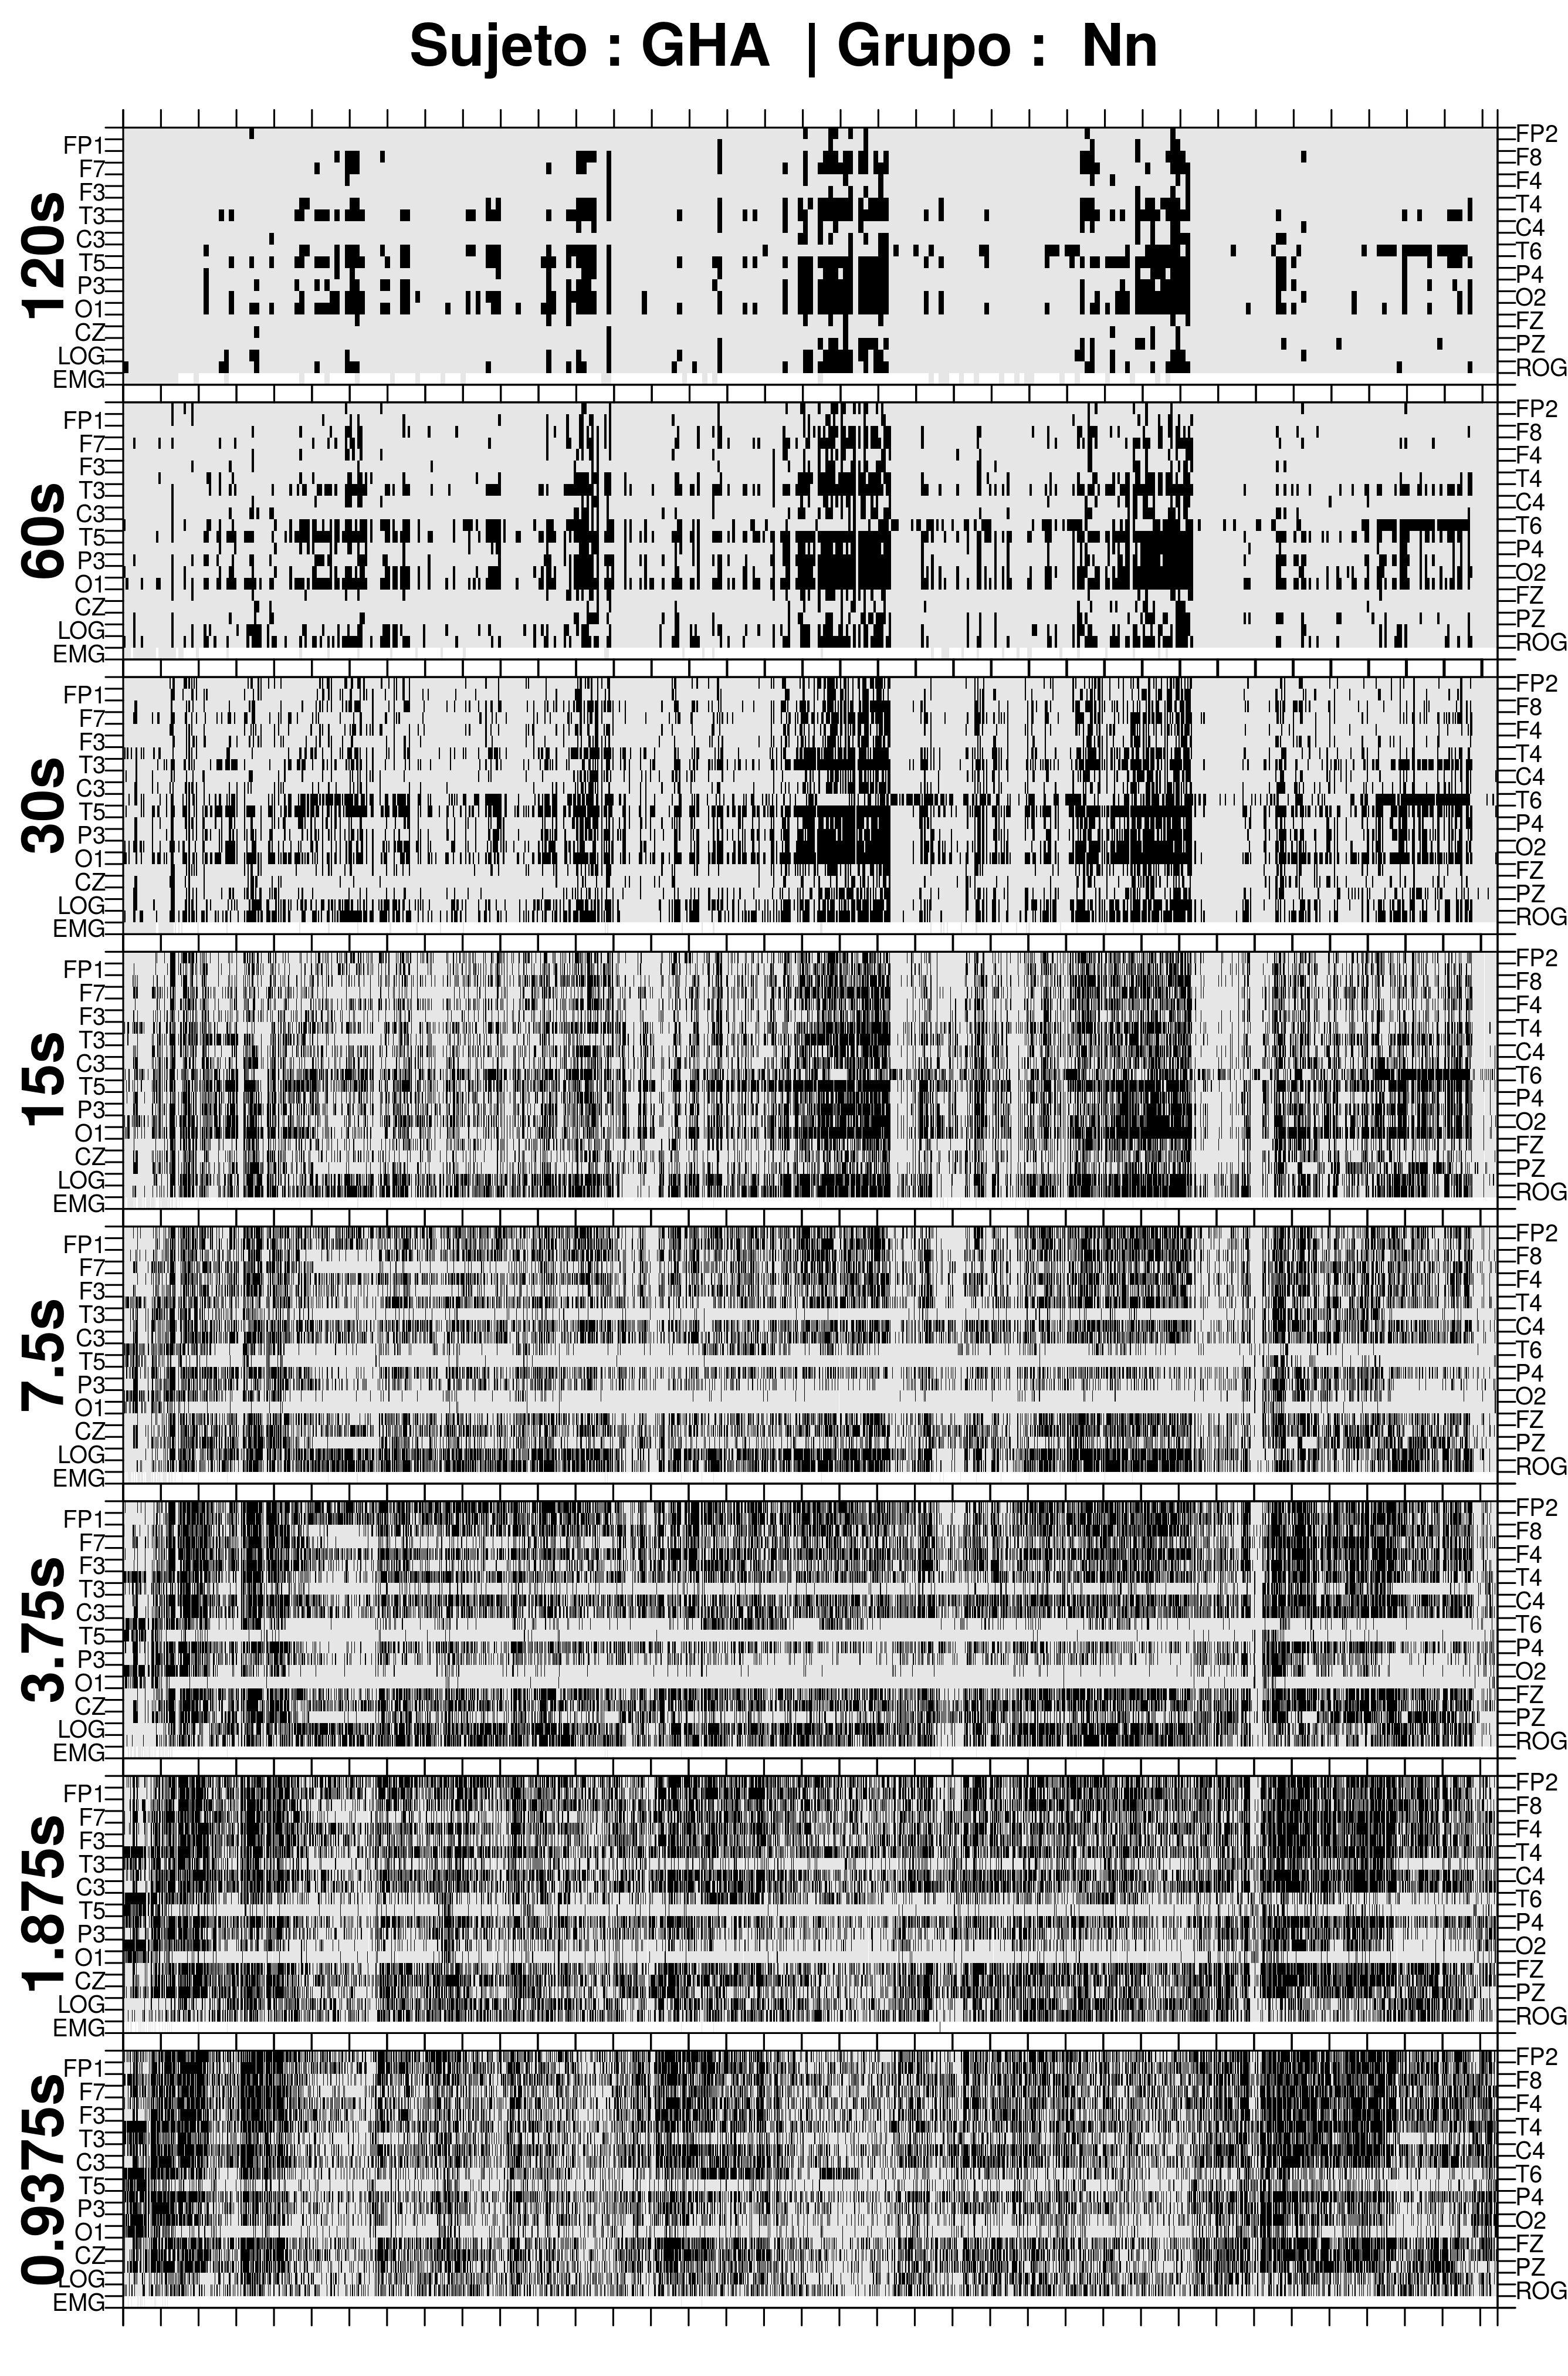
\includegraphics[width=0.9\linewidth]
{./img_ejemplos/GH24031950SUENO_comp_est_.png} 
\end{figure}
\begin{figure}
\centering
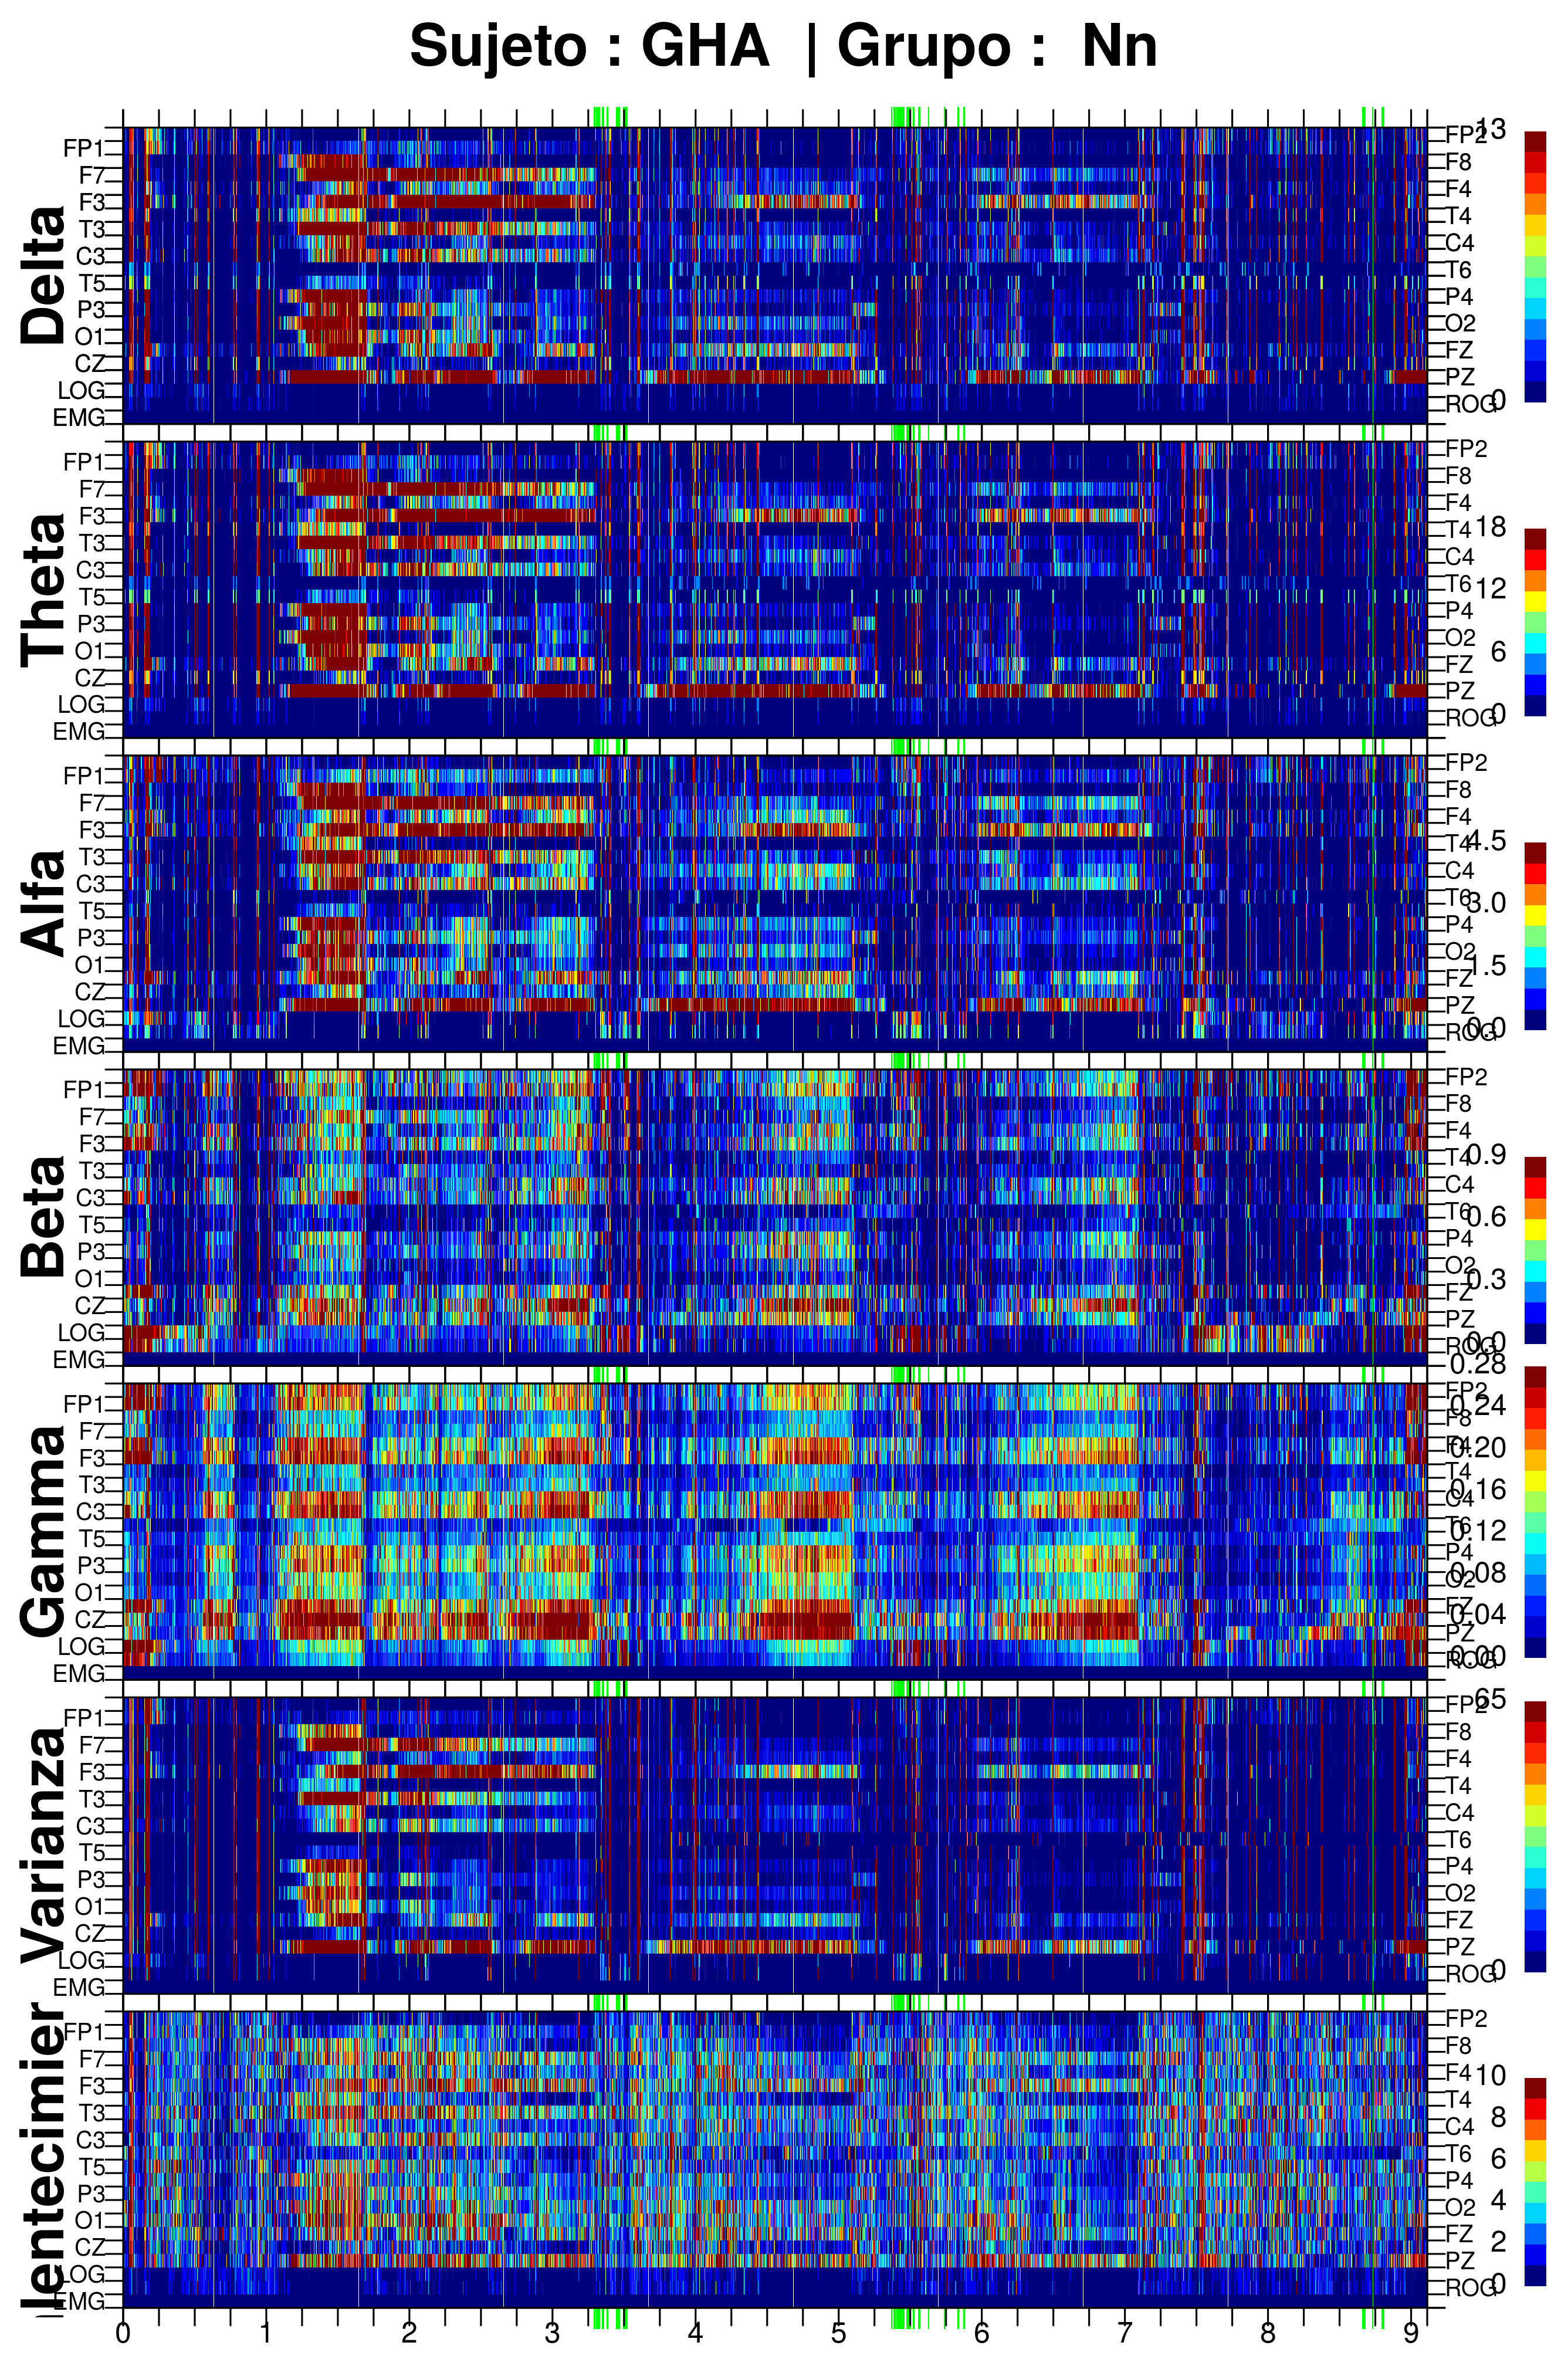
\includegraphics[width=0.9\linewidth]
{./enlentecimiento/GH24031950SUENO_espectral_total.png} 
\end{figure}
\begin{figure}
\centering
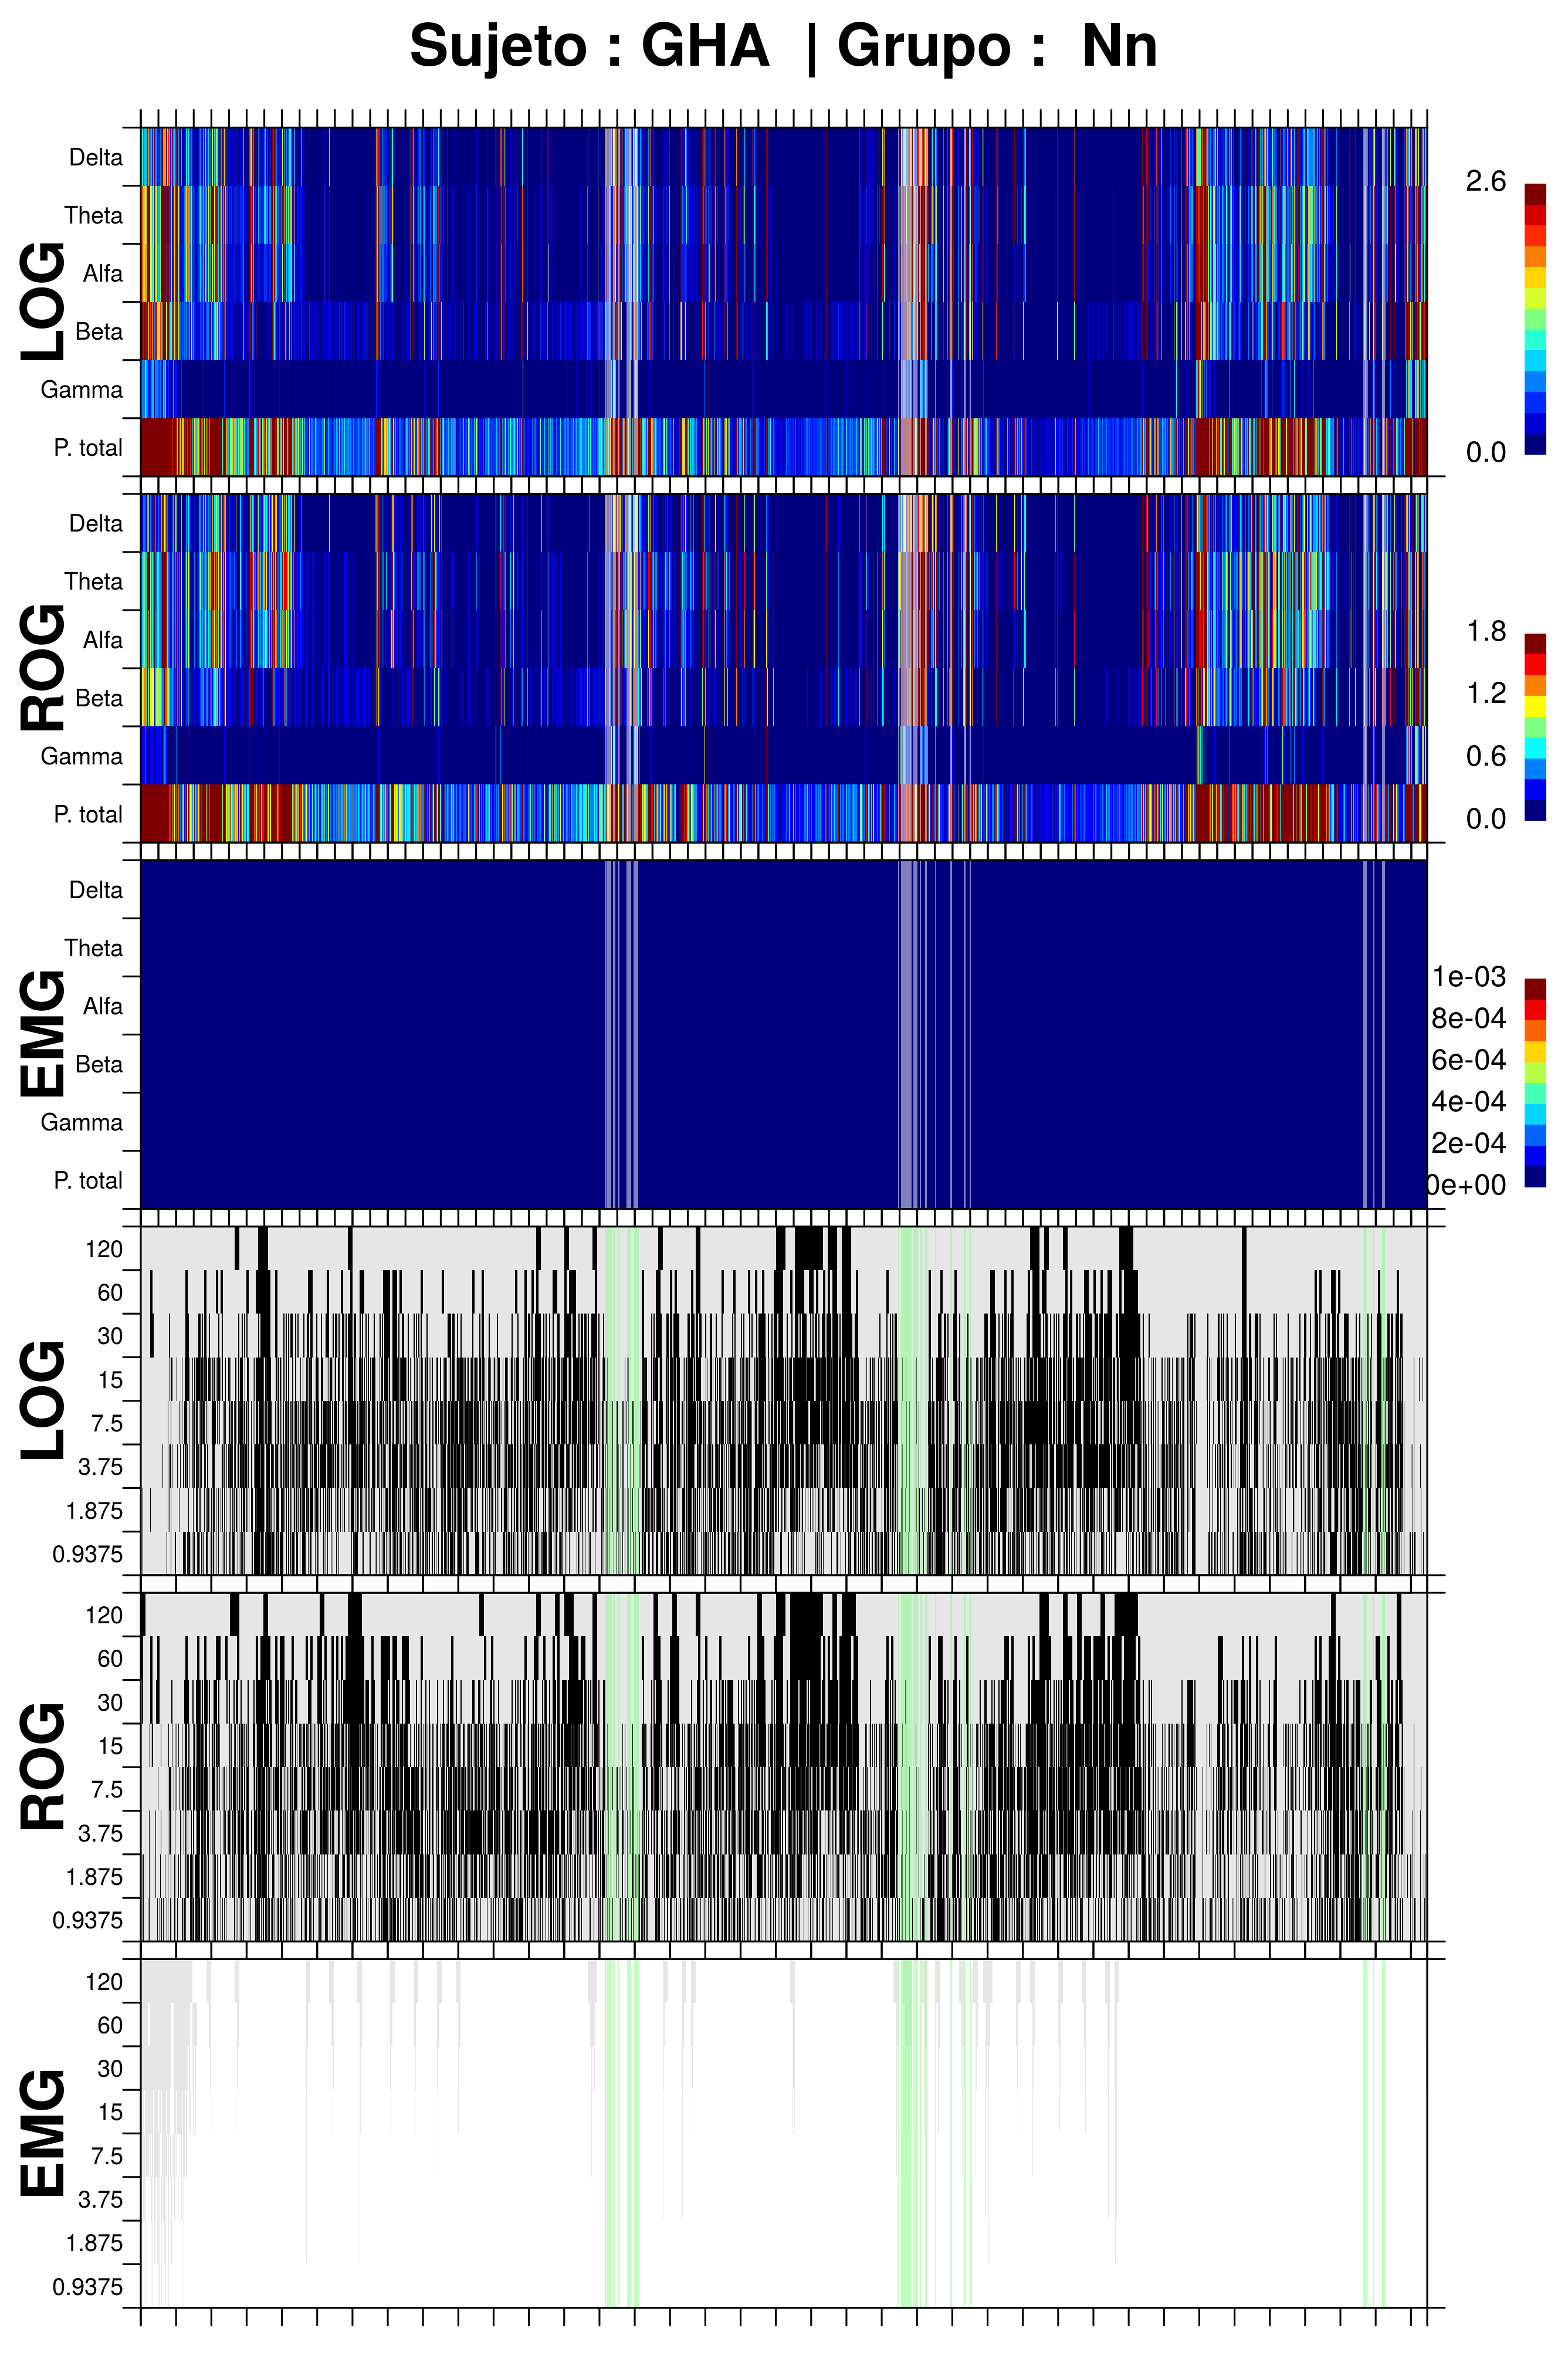
\includegraphics[width=0.9\linewidth]
{./img_resultados/GH24031950SUENO_combinado_.png} 
\end{figure}

\begin{figure}
\centering
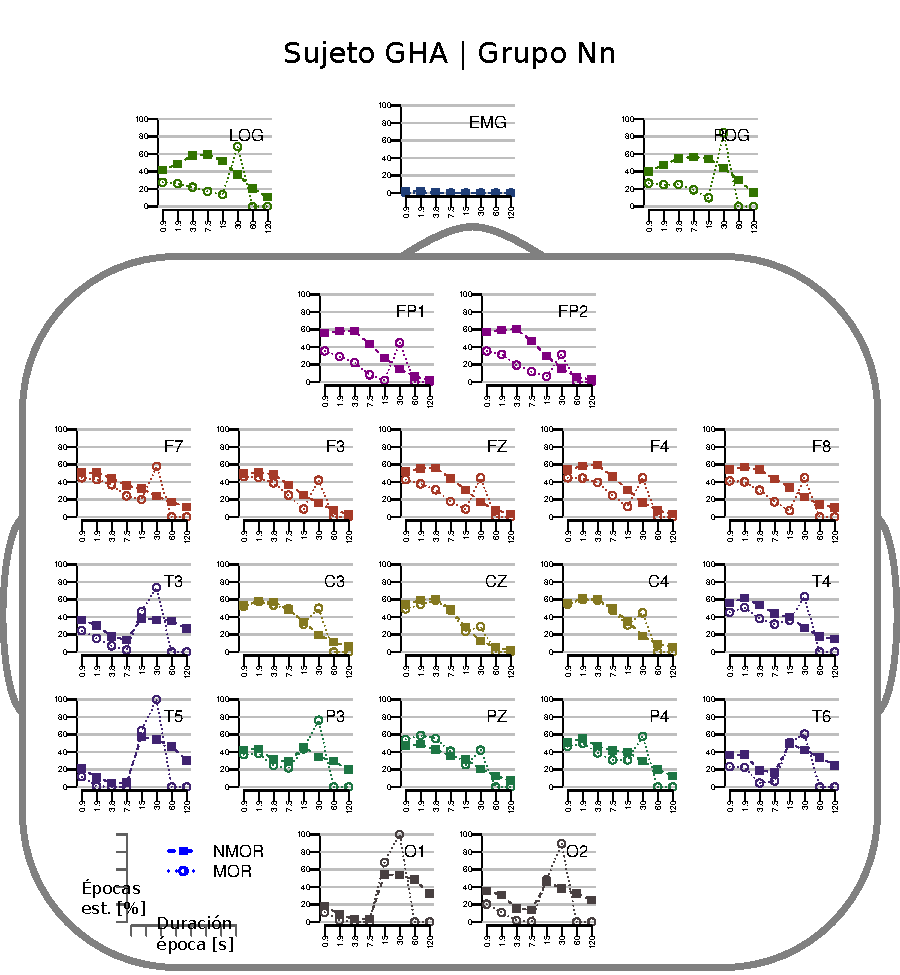
\includegraphics[width=.9\linewidth]{./img_resultados/cabeza_GHA.pdf}
%\caption{Porcentajes de épocas estacionarias, GHA (GH24031950SUEÑO)}
\end{figure}

%%%%%%%%%%%%%%%%%%%%%%%%%%%%%%%%%%%%%%%%%%%%%%%%%

\begin{figure}
\centering
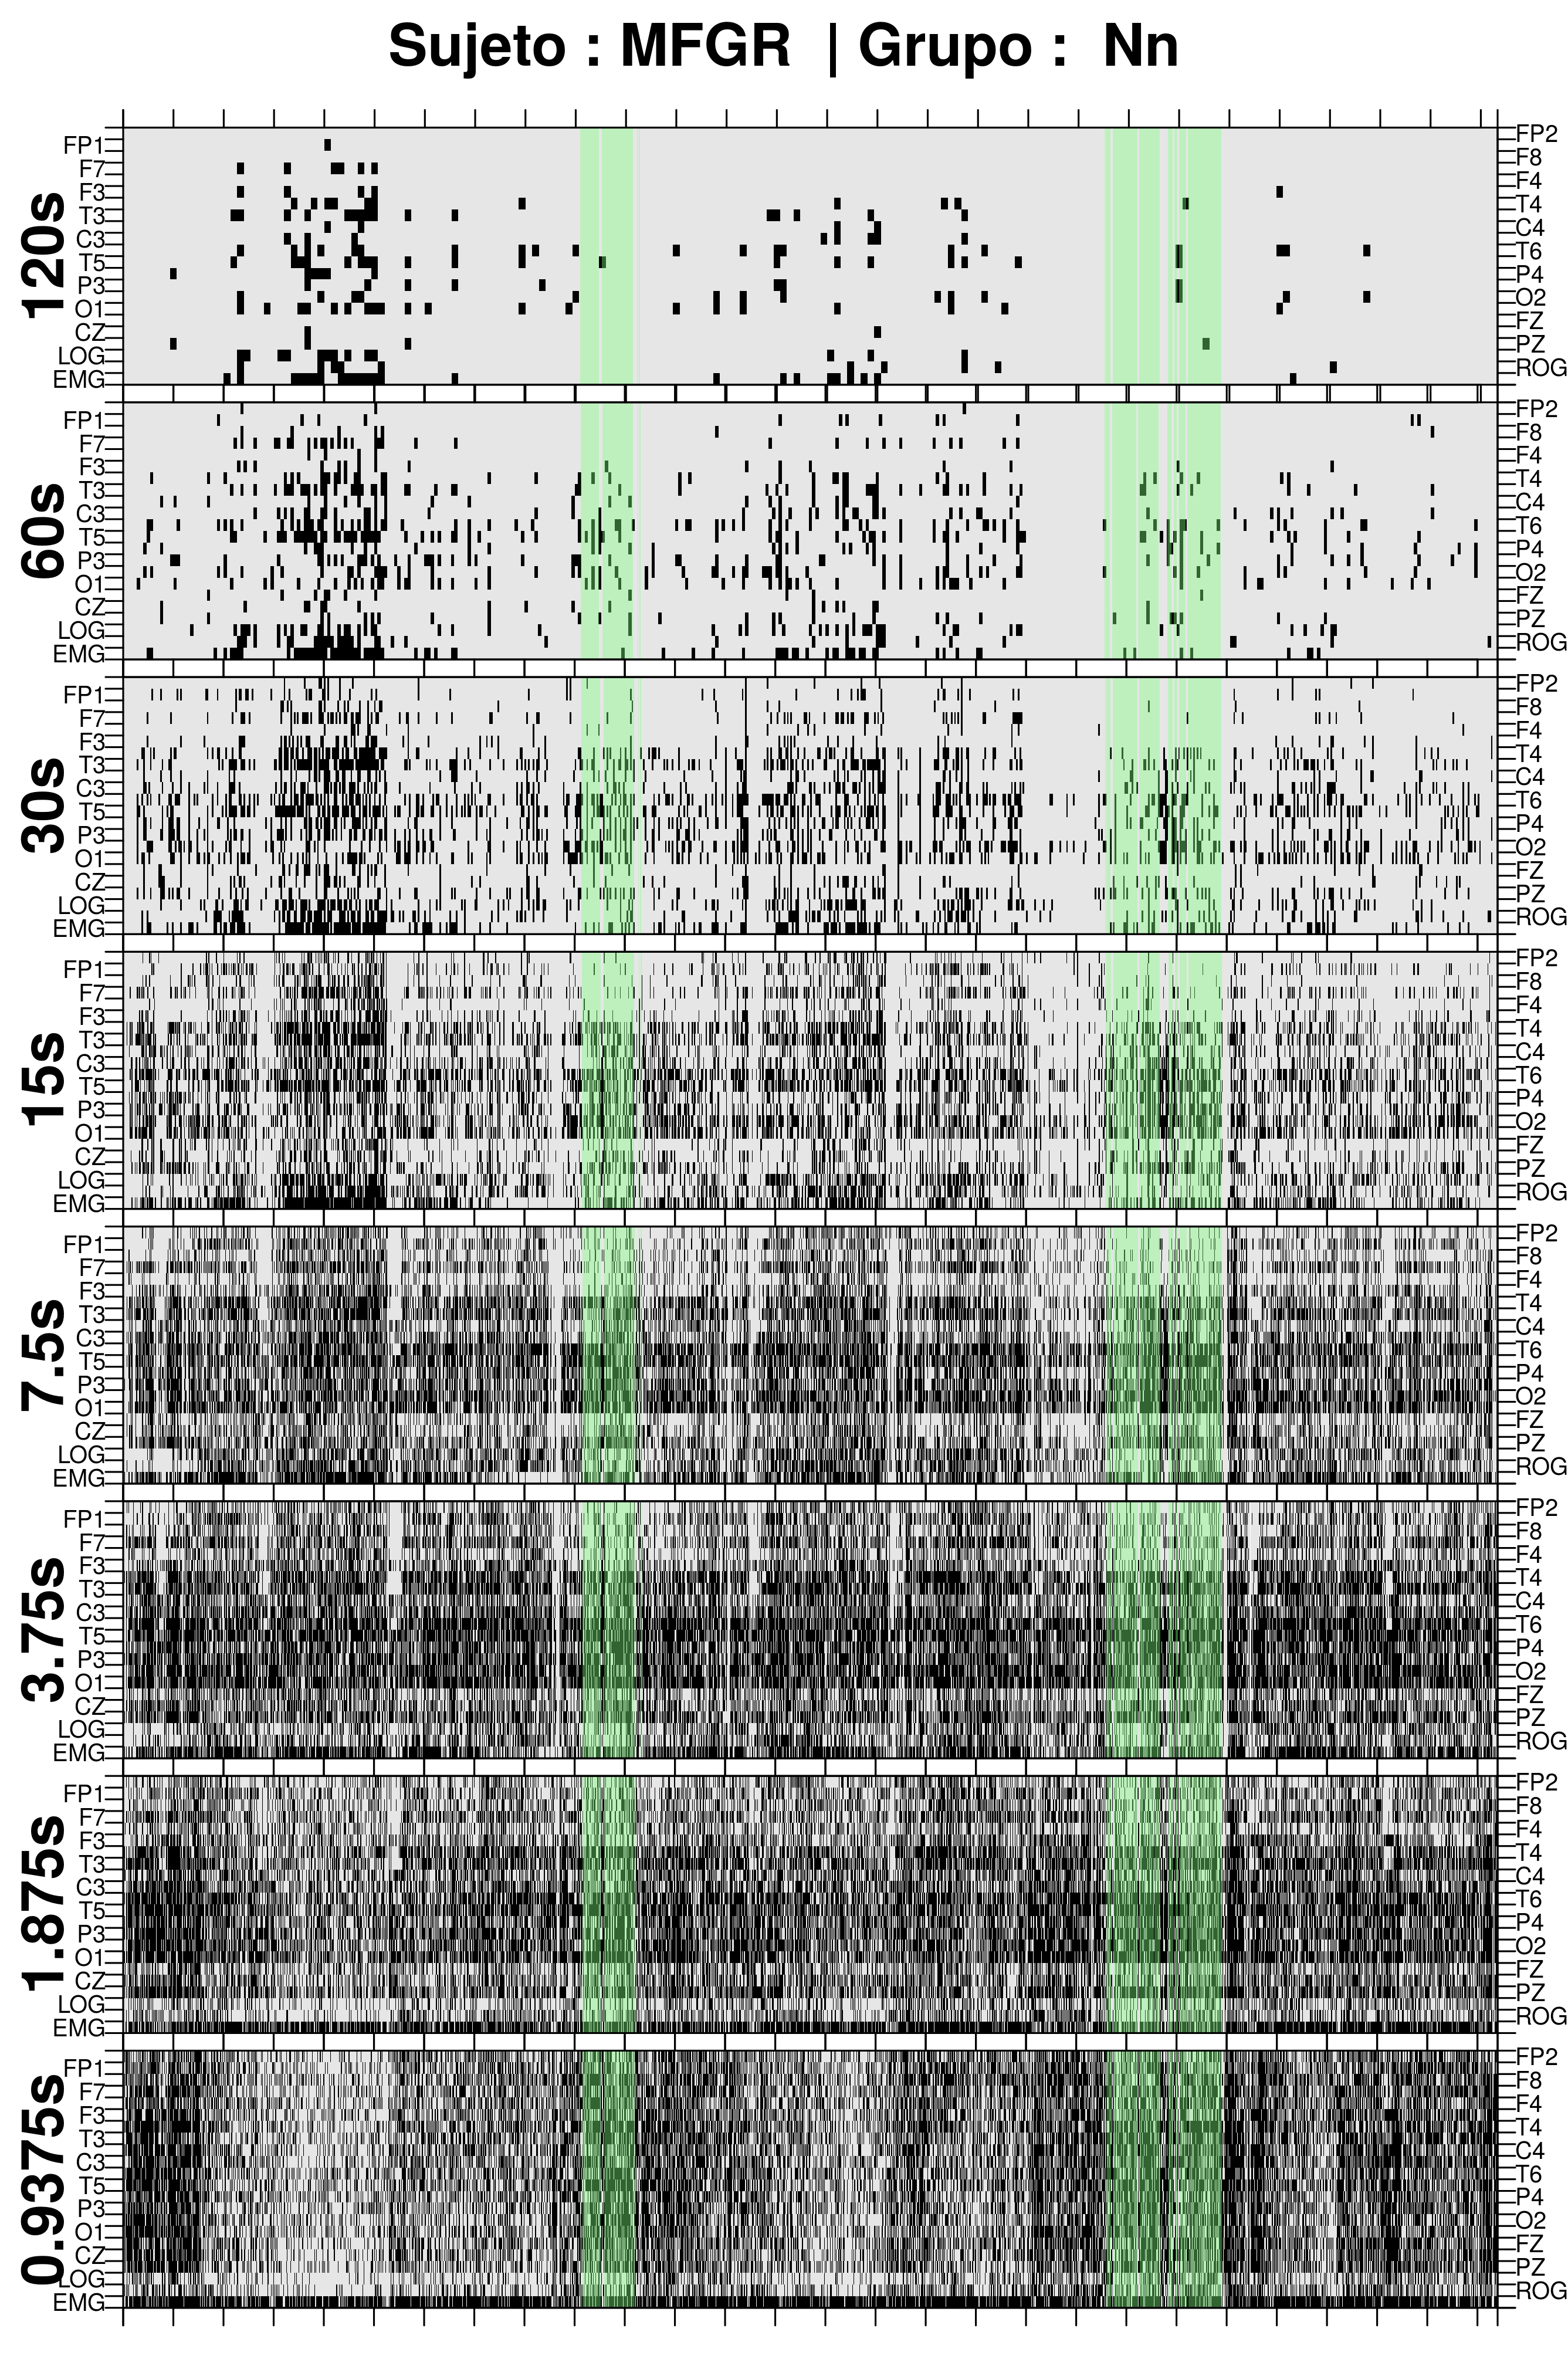
\includegraphics[width=0.9\linewidth]
{./img_ejemplos/GURM251148SUE_comp_est_.png} 
\end{figure}
\begin{figure}
\centering
\includegraphics[width=0.9\linewidth]
{./enlentecimiento/GURM251148SUE_espectral_total.png} 
\end{figure}
\begin{figure}
\centering
\includegraphics[width=0.9\linewidth]
{./img_resultados/GURM251148SUE_combinado_.png} 
\end{figure}

\begin{figure}
\centering
\includegraphics[width=.9\linewidth]{./img_resultados/cabeza_MFGR.pdf}
%\caption{Porcentajes de épocas estacionarias MFGR (GURM251148SUE)}
\end{figure}

%%%%%%%%%%%%%%%%%%%%%%%%%%%%%%%%%%%%%
%%%%%%%%%%%%%%%%%%%%%%%%%%%%%%%%%%%%%
%%%%%%%%%%%%%%%%%%%%%%%%%%%%%%%%%%%%%

\begin{figure}
\centering
\includegraphics[width=0.9\linewidth]
{./img_ejemplos/CLMN10SUE_comp_est_.png} 
\end{figure}

\begin{figure}
\centering
\includegraphics[width=0.9\linewidth]
{./enlentecimiento/CLMN10SUE_espectral_total.png} 
\end{figure}

\begin{figure}
\centering
\includegraphics[width=0.9\linewidth]
{./img_resultados/CLMN10SUE_combinado_.png} 
\end{figure}

\begin{figure}
\centering
\includegraphics[width=.9\linewidth]{./img_resultados/cabeza_CLO.pdf}
%\caption{Porcentajes de épocas estacionarias, CLO (CLMN10SUE)}
\end{figure}

%%%%%%%%%%%%%%%%%%%%%%%%%%%%%%%%%%%%%

\begin{figure}
\centering
\includegraphics[width=0.9\linewidth]
{./img_ejemplos/RLMN10SUE_comp_est_.png} 
\end{figure}
\begin{figure}
\centering
\includegraphics[width=0.9\linewidth]
{./enlentecimiento/RLMN10SUE_espectral_total.png}
\end{figure}
\begin{figure}
\centering
\includegraphics[width=0.9\linewidth]
{./img_ejemplos/RLMN10SUE_comp_est_.png} 
\end{figure}

\begin{figure}
\centering
\includegraphics[width=.9\linewidth]{./img_resultados/cabeza_RLO.pdf}
%\caption{Porcentajes de épocas estacionarias, RLO (RLMN10SUE)}
\end{figure}

%%%%%%%%%%%%%%%%%%%%%%%%%%%%%%%%%%%%%

\begin{figure}
\centering
\includegraphics[width=0.9\linewidth]
{./img_ejemplos/RRMNS_comp_est_.png} 
\end{figure}

\begin{figure}
\centering
\includegraphics[width=0.9\linewidth]
{./enlentecimiento/RRMNS_espectral_total.png}
\end{figure}

\begin{figure}
\centering
\includegraphics[width=0.9\linewidth]
{./img_resultados/RRMNS_combinado_.png} 
\end{figure}

\begin{figure}
\centering
\includegraphics[width=.9\linewidth]{./img_resultados/cabeza_RRU.pdf}
%\caption{Porcentajes de épocas estacionarias, RRU (RRMNS)}
\end{figure}

%%%%%%%%%%%%%%%%%%%%%%%%%%%%%%%%%%%%%

\begin{figure}
\centering
\includegraphics[width=0.9\linewidth]
{./img_ejemplos/JGMN6SUE_comp_est_.png} 
\end{figure}

\begin{figure}
\centering
\includegraphics[width=0.9\linewidth]
{./enlentecimiento/JGMN6SUE_espectral_total.png} 
\end{figure}

\begin{figure}
\centering
\includegraphics[width=0.9\linewidth]
{./img_resultados/JGMN6SUE_combinado_.png} 
\end{figure}

\begin{figure}
\centering
\includegraphics[width=.9\linewidth]{./img_resultados/cabeza_JGZ.pdf}
%\caption{Porcentajes de épocas estacionarias, JGZ (JGMN6SUE)}
\end{figure}

%%%%%%%%%%%%%%%%%%%%%%%%%%%%%%%%%%%%%
%%%%%%%%%%%%%%%%%%%%%%%%%%%%%%%%%%%%%
%%%%%%%%%%%%%%%%%%%%%%%%%%%%%%%%%%%%%

%\begin{figure}
%\centering
%\includegraphics[width=0.9\linewidth]
%{./img_ejemplos/FGHSUE_comp_est_.png} 
%\end{figure}
%\begin{figure}
%\centering
%\includegraphics[width=0.9\linewidth]
%{./img_resultados/FGHSUE_espectral_total.png} 
%\end{figure}
%\begin{figure}
%\centering
%\includegraphics[width=0.9\linewidth]
%{./img_resultados/FGHSUE_combinado_.png} 
%\end{figure}
%
%\begin{figure}
%\centering
%\includegraphics[width=.9\linewidth]{./img_resultados/cabeza_FGH.pdf}
%%\caption{Porcentajes de épocas estacionarias, FGH (FGHSUE)}
%\end{figure}

%%%%%%%%%%%%%%%%%%%%%%%%%%%%%%%%%%%%%

%\begin{figure}
%\centering
%\includegraphics[width=0.9\linewidth]
%{./img_ejemplos/MGNA5SUE_comp_est_.png} 
%\end{figure}
%\begin{figure}
%\centering
%\includegraphics[width=0.9\linewidth]
%{./img_resultados/MGNA5SUE_espectral_total.png} 
%\end{figure}
%\begin{figure}
%\centering
%\includegraphics[width=0.9\linewidth]
%{./img_resultados/MGNA5SUE_combinado_.png} 
%\end{figure}
%
%\begin{figure}
%\centering
%\includegraphics[width=.9\linewidth]{./img_resultados/cabeza_MGG.pdf}
%%\caption{Porcentajes de épocas estacionarias, MGG (MGNA5SUE)}
%\end{figure}

%%%%%%%%%%%%%%%%%%%%%%%%%%%%%%%%%%%%%

%\begin{figure}
%\centering
%\includegraphics[width=0.9\linewidth]
%{./img_ejemplos/EMNNS_comp_est_.png} 
%\end{figure}
%\begin{figure}
%\centering
%\includegraphics[width=0.9\linewidth]
%{./img_ejemplos/EMNNS_comp_est_.png} 
%\end{figure}
%\begin{figure}
%\centering
%\includegraphics[width=0.9\linewidth]
%{./img_ejemplos/EMNNS_comp_est_.png} 
%\end{figure}
%
%\begin{figure}
%\centering
%\includegraphics[width=.9\linewidth]{./img_resultados/cabeza_EMT.pdf}
%%\caption{Porcentajes de épocas estacionarias EMT (EMNNS)}
%\end{figure}

%%%%%%%%%%%%%%%%%%%%%%%%%%%%%%%%%%%%%

%\begin{figure}
%\bordes{1.5}
%\begin{tabular}{l}
%\Large{{Patrones visuales}}\\
%\begin{tabular}{c}
%\includegraphics[width=0.45\textwidth]
%{./img_ejemplos/zoom_VCR.pdf}
%\includegraphics[width=0.45\textwidth]
%{./img_ejemplos/zoom_MJH.pdf}
%\\
%\includegraphics[width=0.45\textwidth]
%{./img_ejemplos/zoom_JAE.pdf}
%\includegraphics[width=0.45\textwidth]
%{./img_ejemplos/zoom_GHA.pdf}
%\\
%\includegraphics[width=0.45\textwidth]
%{./img_ejemplos/zoom_MFGR.pdf}
%\end{tabular}
%\end{tabular}
%\end{figure}

%%%%%%%%%%%%%%%%%%%%%%%%%%%%%%%%%%%%%%%%%%%%%%%%%%%%%%%%%%%%%%%%%%%%%%%%%%%%%%%%%%%%%%%%%%%%%%%%%%%
%%%%%%%%%%%%%%%%%%%%%%%%%%%%%%%%%%%%%%%%%%%%%%%%%%%%%%%%%%%%%%%%%%%%%%%%%%%%%%%%%%%%%%%%%%%%%%%%%%%
%%%%%%%%%%%%%%%%%%%%%%%%%%%%%%%%%%%%%%%%%%%%%%%%%%%%%%%%%%%%%%%%%%%%%%%%%%%%%%%%%%%%%%%%%%%%%%%%%%%
%%%%%%%%%%%%%%%%%%%%%%%%%%%%%%%%%%%%%%%%%%%%%%%%%%%%%%%%%%%%%%%%%%%%%%%%%%%%%%%%%%%%%%%%%%%%%%%%%%%
